\documentclass[11pt, twoside, reqno]{book}
\usepackage{amssymb, amsthm, amsmath, amsfonts}
\usepackage{graphicx}
\usepackage{color}
\usepackage{url}
\usepackage{hyperref}
\usepackage{verbatim}
\usepackage{ wasysym }
\usepackage{pdfpages}
\usepackage[toc,page]{appendix}
\appendixpageoff
\usepackage[leftmargin = 1in, rightmargin = 0in, vskip = 0in]{quoting}
\usepackage{microtype}
\usepackage{bardtex}
\styleoption{seniorproject}
\usepackage{listings}
\definecolor{codegreen}{rgb}{0,0.6,0}
\definecolor{codegray}{rgb}{0.5,0.5,0.5}
\definecolor{codepurple}{rgb}{0.58,0,0.82}
\definecolor{backcolour}{rgb}{0.95,0.95,0.98}
\lstdefinestyle{mystyle}{
    commentstyle=\color{codegreen},
    keywordstyle=\color{magenta},
    stringstyle=\color{codepurple},
    basicstyle=\ttfamily,
    backgroundcolor=\color{backcolour},
    frame=lrbt,
    breakatwhitespace=false,      
    framexleftmargin=8pt, 
    framexrightmargin=8pt,   
    framextopmargin=6pt,
    framexbottommargin=6pt,
    breaklines=true,                 
    keepspaces=false,                 
    numbersep=0pt,                  
    showspaces=false,                
    showstringspaces=false,
    showtabs=false,                  
    tabsize=1
}
\lstset{style=mystyle}
\newcommand{\blockquotespacing}{\blockspaced}
\newcommand{\prose}{.25in}
\newcommand{\poetry}{0in}
\newcommand{\singlespaced}{\setstretch{1}\vspace{\baselineskip}}
\newcommand{\blockspaced}{\setstretch{1.3}\vspace{\baselineskip}}
\newcommand{\doublespaced}{}
\newenvironment{blockquote}[1][\prose]{\setlength{\parindent}{#1}\begin{quoting}\blockquotespacing}{\end{quoting}}
\begin{document}

\titlepg{Determining Tone of a Body of Text}{Cole Hollant}
    {May}{2020}

\abstr
We will be looking into emotion detection and manipulation within a body of text based off of Robert Plutchik's basic emotions. This project encompasses building probabilistic and lexical models, full-stack web development, and dataset creation and application. We will build our models off of Latent Dirichlet Allocation—a grouping model common in natural language processing (nlp) and lexicons compiled through crowdsourcing. User testing is undergone as a means of measuring the effectiveness of our models. We discuss the application of concepts and technologies including MongoDB, REST APIs, containerization, IaaS, and web frontends.

\tableofcontents

\dedic

% Dedicated to Jeff and Joel, wouldn't have made it here without you :)
Dedicated to Sawyer. I love you more than anything; I do it all for you, buddy

\acknowl

Thank you to all of my beautiful friends, from school and from home. A special thanks to:

\begin{itemize}
  \item Emma, for getting me through higher education—my maths partner-in-crime
  \item Brooke, Mary, Thea, and Laina for being my rock throughout all these years
  \item  Cullen, for all the nights by the CRT, and for being there when I was the biggest mess I've ever been
  \item  Ariadne, for lighting up RKC for me every day
  \item Tim, Hanna, Zyrene, and Andi, my wonderful dev family, you've more or less got me to where I am today
  \item Theo and Kaylin, you two are my home away from home
\end{itemize}

And of course, thank you to my wonderful family. You have given me everything. I love you :)

\startmain

\intro

This project is twofold, encompassing natural language processing (nlp) and full stack web development. Regarding nlp, we are in the realm of emotion analysis as we seek to algorithmically discern emotion within text. We largely take our conceptions of emotion from Robert Plutchik.

\begin{figure}[h!]
  \centering
  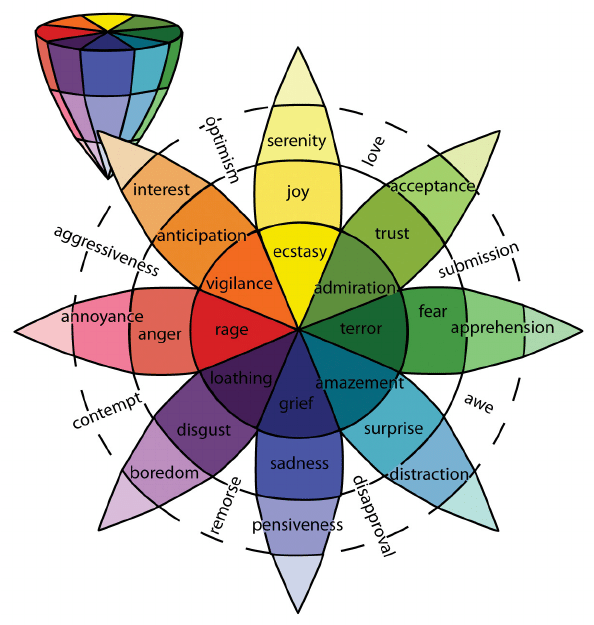
\includegraphics[width=15cm, height=6cm, keepaspectratio]{plutchikWheel.png}

  {\small \textit{Plutchik's Wheel} \cite{Plutchik7:online}}
  \caption{
    Emotion is a complex chain of loosely connected events that begins with stimulus and includes feelings, psychological changes, impulses to action and specific, goal-directed behavior. \cite{10.2307/27857503}
  }
  \label{fig:wheel}
\end{figure}


Plutchik's wheel of emotions \ref{fig:wheel} relates to color theory, such that an emotion can be seen as a mixture of emotions (i.e. ``anticipation'' lays between ``joy'' and ``anger''). The core pillars of emotion are joy, trust, fear, surprise, sadness, disgust, anger, and anticipation. Due to lexical limitations, our models will only be based off of anger, sadness, joy, and fear. Emotion detection within text is a rather difficult problem, although it has grown in popularity recently. The dichotomy between difficulty and popularity results in what Seyeditabari et al. articulate as insufficient datasets \cite{DBLP:journals/corr/abs-1806-00674}. They mention several available datasets, as well as different methods in use, including the affect dataset from Mohammad and Turney \cite{Mohammad13} that we use; the methods noted fall into the supervised and unsupervised categories. The supervised methods include data collection through Twitter scraping and large surveys, as well as their use within support vector machines (SVM), naive Bayes classifiers, and $k$-nearest neighbor (KNN) clustering. The unsupervised methods include Probabilistic Latent Semantic Analysis (PSLA), simple lexical approaches, and point-wise mutual information (PMI) \cite{DBLP:journals/corr/abs-1806-00674}. We will make two unsupervised models for emotion detection based on our subset of emotions from Plutchik's wheel; the first model will take a lexical approach, where we take the average token scores for each affect based on Mohammad and Turney's word-affect and affect-intensity lexicons; the second will be based on Latent Dirichlet Allocation (LDA), a generalization of PSLA by Blei et al. \cite{david_m._y._i._1970}. In addition to our two emotion-detection models, we look into word replacement models based on a thesaurus \cite{BigHugeT88:online} and our scoring models. One such model performs arbitrary replacement based on synonyms of tokens; the other seeks to maximize score in one of our affect categories.

A large focus was placed on full-stack web development: dataset creation/consumption, database management, server configuration, creating REST APIs, and creating a web frontend. We leverage several technologies for this, including Python with Flask \cite{Welcomet33:online}, Golang and the mongo-go-driver \cite{mongogod83:online}, HTML/CSS/Javascript via VueJS \cite{Vuejs17:online}, and Docker \cite{Empoweri41:online}.
\newpage
\begin{figure}[h!]
  \centering
  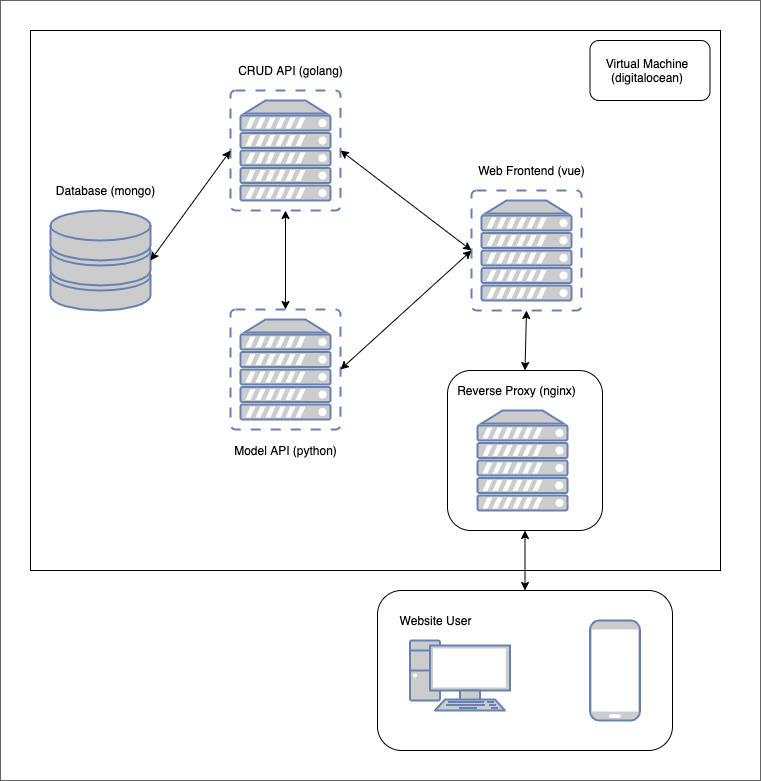
\includegraphics[width=15cm, height=12cm, keepaspectratio]{architecture.png}
  
  \caption{architecture diagram}
  \label{fig:architecture}
\end{figure}

Figure \ref{fig:architecture} serves to describe our application. Once a user requests our site, our reverse-proxy forwards this request to our frontend server. Then, when the user accesses the thesaurus page, they see results from calling our CRUD-wrapper API that accesses our database. When they use the models on the site they are making requests to the model API—which then makes requests to the CRUD API. For scalability, ease of deployment, and security benefits, the frontend, model API, CRUD API, and database are all in containers. All of this sits on a virtual machine from DigitalOcean \cite{DigitalO1:online}, with the code available on Github \cite{GitHub86:online}.

% We will begin discussing server configuration, move to database construction, then our CRUD API, followed by our models, the frontend, and finishing with results.
This paper will discuss the design and implementation of emotion detection and manipulation based on our subset of Plutchik's basic emotions and user-tested sentiment. In chapters two and three respectively, we discuss server configuration and database construction. Next, in chapter four, we discuss the implementation and usage of our CRUD-wrapper API. Finally, in chapters five and six, we define our models and present a frontend that allows for user interaction. Results and next steps are discussed in the context of our experiment in chapters seven and eight.

























\chapter{Hosting}

The first step in implementing the defined architecture is discussing our options for hosting our services; this will necessitate some sort of server. While we \textit{could} do everything locally to save some of the configuration headache, this limits the accessibility of our application to those that can access our repository and recreate our project. In the pursuit of functionality, accessibility, and thoroughness, we will need a server to put this on.

\section{Server Options}

After ruling out \texttt{Make} as our distribution strategy, we still have several options for this project in terms of hosting. These options come as a slew of acronyms: IaaS, PaaS, and I suppose some bare-metal solution could work. The last option would consist of a computer running 24/7 in my dorm room, along with some router configurations that might have the college's IT department knocking at my door, thus leaving the others as the real contenders. There's a certain balance between PaaS (Platform as a Service) and IaaS (Infrastructure as a Service), each with some pros and some cons. IaaS can provide an experience similar to working on your own computer; it is as close to the bare-metal (often called ``on-premises'') solution as possible, where we would pay for a virtual machine (VM) and networking. With IaaS we are leveraging server farms, and are more-or-less renting a server. PaaS is more nuanced, as it plays a role between IaaS and SaaS (Software as a Service, like Google Apps, Dropbox, etc.), and tends to abstract desirable aspects of IaaS such as security, metrics, DNS, and so on.

We ultimately went with IaaS via DigitalOcean \cite{DigitalO1:online}, a popular cloud services platform among names like AWS, GPC, and Azure. This gives us the development advantage of having all our services in the same place—allowing us to more easily build and tear down our project—as opposed to the spread out nature of PaaS. There are exceptions to this heuristic, such as Kubernetes, Openshift, and other CaaS (Containers as a Service) platforms, that would allow us to keep centralized services, but pricing is one of the biggest sellers for our use of IaaS. We lose some of the ease of scalability, but that is not an aspect that we are terribly concerned with while developing the core of the project. As we went with IaaS, we will get our hands dirty with SSL, proxies, and other niceties that PaaS would shield us from.

It should go without saying that it's wise to stray from doing all things as the \texttt{root} user. By default, we can only \texttt{ssh} into \texttt{root}, and in order to get around this, we will have to add a user. We'll still need administrative access, so we'll be sure to add our new user to the \texttt{sudo} group. Then to finish our user setup, we must patch up our \texttt{ssh} configuration: we want to \texttt{ssh} as the created user and disable \texttt{ssh} for \texttt{root}.

\begin{figure}[h!]
\begin{lstlisting}[language=sh]
ssh root@<IP_ADDRESS>
adduser <USERNAME>
usermod -aG sudo <USERNAME> 
rsync --archive --chown=<USERNAME>:<USERNAME> ~/.ssh /home/<USERNAME> 
vim /etc/ssh/sshd_config    # (set "PermitRootLogin" to "no")
\end{lstlisting}
\caption{Adding a new user, and removing \texttt{ssh} access for \texttt{root}}
\end{figure}

As a convenience, we will add an \texttt{ssh} config on our personal machine. This saves the hassle of keeping track of IP addresses and users and keys, then we can enter through the name of the entry \texttt{ssh <entry-name>}.

\section{Containerization}

Containers are an industry-molding alternative to virtual machines for running OS agnostic programs. We are using Docker to deploy each of our services; Docker is a wildly popular open source project for creating, distributing, and running containers.

\begin{figure}[h!]
  \centering
  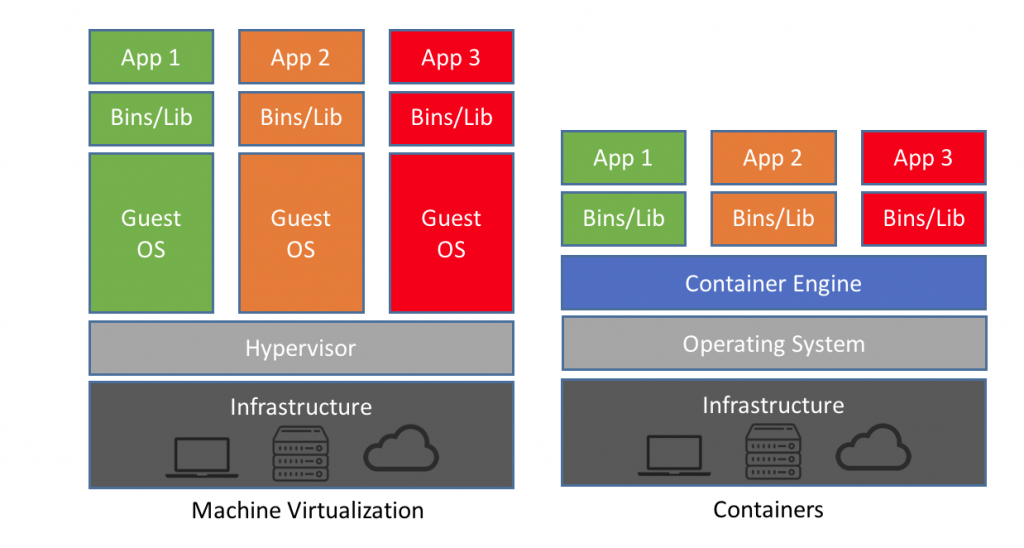
\includegraphics[width=125mm,scale=0.5]{dockerImage.png}
  
  \caption{Dockerization vs Containerization \cite{ScreenSh29:online}}
  \label{fig:docker}
\end{figure}

On each side of figure \ref{fig:docker}, we have a layer of apps on top of their dependencies, all of which run on top of some infrastructure. The apps and ``bins/libs'' are our binaries/executables/processes along with their source-code/libraries that we are used to writing and running in our day-to-day as programmers. The infrastructure is just that: the silicon and bare metal that we are running on top of. That wraps up the local development experience, which has drawbacks when it comes to distribution/deployment.

The ``it worked on \textit{my} computer'' dilemma is what virtualization and containerization are here to address. Platform-independent programs result from the abstraction of these processes and dependencies from the contents of their user space. Virtual machines tackle this by building entire guest operating systems on top of a hypervisor (also known as a virtual machine monitor), which serves to channel access to hardware and thus allow for multiple operating systems to run on one host operating system.

However, operating systems are quite large, and there is a lot of waste with virtualization. With the industry going towards cloud computing, we needed smaller, faster solutions. Containerization seeks to leverage the host operating system, and rather than keep several guest-os instances, we have a single container runtime environment. This is a similar solution to that which the JVM provided in the 1990's: the program is to run on a layer that is abstracted from the OS. This then begs the question of whether the JVM is necessary within the context of containerization: if we can specify the ``machine'' that our program is run on in a replicable fashion, what purpose does the JVM serve? This gets at a core problem of containerization, in that we want to have our containers as small as possible. This way we save on resources, and—in the case of serverless architecture—speed.

This may not seem all that important, as we are only talking on the order of megabytes. But in the days where serverless architecture/microservices are growing in popularity, there is an ever-increasing need for quick cold-start times (starting an idle container, should none be active and available). Serverless computing being a platform in which cloud providers provision your resources, and the customer is charged for active time rather than paying for a more traditional fixed-rate server. This is attractive as it isn't wasteful and is incredibly scalable, but there's always a chance that your containers are down when a request is made; in the event that we have a cold start, the containers must be reinitialized to fulfill the request. Additionally, containers must share their host's kernel, which means that they cannot be \textit{as} secure as virtual machines, which is something that we have to take into consideration.

\subsection{Defining Containers}

With containerization, the name of the game is modularity; we generally aspire to have per-process containers. Given this per-process goal, we will need to have a container for each independent service of our application, thus my one web app comprised of a frontend, a database, a CRUD-wrapping API, a model API, and a server/reverse-proxy has five containers: one for each aspect. With inter-container dependencies, we see a similar struggle arise with the management of individual containers. Docker-compose is a tool that allows for the definitions/instructions for multiple containers, allowing us to deploy our application with a single command. This is specified in a \texttt{yaml} file and maps nicely to standard docker cli arguments. We note things like \texttt{Dockerfile} location, port forwarding, networks, inter-container dependencies, volumes, environment variables and so on. These are necessary as a means of communicating between the host and the container, between the containers themselves, and for the preservation of data once a container is killed.

\label{Go CRUD API Dockerfile}

Golang compiles to binaries per OS, which is excellent news for us! If we can compile to binaries, we don't need to keep all the installation business around, so we simply copy over the source code, install the packages, and compile as a build stage. Then we can copy over the executable to a smaller base image, expose our port, and run! It's a process similar to a writing standard shell script, and we are generally concerned with the resulting size. This was an example of a multistage Dockerfile, where we separate the compilation stage from the runner stage; this is quite common as a measure of reducing image size.

\label{Python Model API Dockerfile}

The Python Dockerfile took was initially very straightforward, but additional modules led to a rewrite. In the beginning, it was more or less copying our files, running \texttt{pip install -r requirements.txt}, exposing a port, and running. Adding \texttt{gensim} as a dependency required certain libraries not present in our Alpine base image (Alpine being a remarkably small linux distribution). We ultimately switched to a different base image to avoid some of the guesswork involved in tracking down the missing dependencies, although if we were to place a bigger priority on container performance, there are strategies for reducing the size of Python containers. Among these are compiling with Cython and \texttt{pip install}-ing your code base \cite{Multista76:online}.

\label{Vue Frontend Dockerfile}

The Dockerfile for the frontend is refreshingly simple. We copy over the source code, install all the dependencies, and build our app. Then we follow our example from the Golang container and run the webserver from a smaller nginx image. We install the Vue CLI tools separately from the other node dependencies. This is because docker caches intermediate image tags per layer (each line in the Dockerfile), which we may run from; there is thus a balance between giving more steps for debugging and writing compact steps to save space.

\label{Mongo and Nginx}

The MongoDB and Nginx containers are as easy as can be. We change nothing from the base images! We just interface with them through container properties, specifying ports, environment variables, etc.

\label{Composition}

Within our docker-compose file, we naturally define a service for each previously mentioned aspect. The common pieces are that each service is given the location of the Dockerfile or image, all are set to restart unless-stopped (as we will only be deploying a single instance of this), each is given a tty in case anything goes wrong, each service is given a port mapping, and everything is added to a network. Outside of this, we link the Golang container to the database, and we are good to go! From here we can build our cluster, run it, and tear it down at will, all by running \texttt{docker-compose build | up | down}.

Since this deployment is in essence a personal project, we won't be concerned with auto-scaling and load-balancing. Should the need arise, everything is fully containerized, and it is just a matter of migrating to a container orchestration platform like Kubernetes.







\chapter{Database Creation}

We are using MongoDB \cite{Themostp65:online} as our database. This is a NOSQL, document-based database that uses BSON (binary JSON). The databases are organized into collections of documents, where collections are analagous to tables, and documents are self-describing entries. We have five collections: \texttt{affectintensity}, \texttt{color}, \texttt{senselevel}, \texttt{vad}, and \textt{words}. The first four are from lexicons sourced from Mohammad and Turney \cite{Mohammad13}, and the \texttt{words} collection was scraped from an online thesaurus \cite{BigHugeT88:online}.

\section{Thesaurus}

As we are building models to analyze/alter the tone of a body of text while attempting to preserve semantics, we suppose that swapping a word for a synonym may alter the tone of its enclosing sentence. Consequently, we would like to aggregate some relative relationship between some set of tones and groups of synonymous words. Upon creating such a dataset, we may interchange a word with a synonym according to a difference in tone: the sentence "That person is cool." may carry a different tone that "That person is unemotional."

\subsection{API Choice}

% First and foremost, we are interested in keeping additional data regarding tone that is not present within existing thesaurus APIs. It is far easier to manipulate data if it is all on hand, and it should save some server-side complexity in dealing with the decoupling of the thesaurus and the word-tone relationships.

There are a few reasons to construct or reconstruct our own thesaurus. First and foremost, this allows us to add and remove entries at will, rather than relying on existence within a third-party dataset; this becomes more important with word processing where we would like to store word-stems with the words themselves. There is an issue with cost as well: APIs are rarely free past some established number of calls in a given time interval or may be free only for a period of time. This software will function with minimal cost—ideally the only cost is in hosting. Finally, this is a project in the realm of software engineering; while it is often better to rely on existing services—standing on the shoulders of those who came before you—it is also important to know how to create your own services.

\subsection{Implementation}

We created the thesaurus by web scraping, which is a large aspect of data-collection and thus is often a necessity in the sphere of machine learning. Of course, it is possible to compile a thesaurus using other means—surely one could buy a physical thesaurus and type up all the entries or even automate such tasks with OCR—, but we are interested in constructing a thesaurus as painlessly as possible—it is only one aspect of our project after all.

\subsubsection{Choosing a site}

Web scraping often comes with a give and take. There are several existing online thesaurus services, and after careful review we landed on John Watson's Big Huge Thesaurus \cite{BigHugeT88:online}. We began with trying \href{https://www.thesaurus.com}{thesaurus.com} \cite{Thesauru2:online}, but they have protections against traditional scraping. There are many of such protections including lazy-loading content, providing fake data, gating with services like Captcha, even automatically altering the page's HTML. It seemed as if \href{https://www.thesaurus.com}{thesaurus.com} had been randomizing their CSS classes and either lazy-loading content or providing fake data. While we could likely get around this with an automated browser like Selenium \cite{Selenium25:online}, as the CSS classes are only a deterrent if scraping over a large time interval and the content would almost certainly exist within an automated browser session, we should respect that this site has practices in place to prevent scraping.

There may be protections against web scraping in place that we ought to honor, or there are often poorly laid out websites that would be a pain to use despite being open source, or the site may simply not provide all the information we would like. The latter is best exemplified by moby \cite{MobyThes97:online} which we may come back to if we decide that we care not about parts of speech. John Watson's Big Huge Thesaurus \cite{BigHugeT88:online}, on the other hand, seems to have all that we want: synonyms by part of speech, a clean interface, and permission for use given credit is provided. \cite{HowToPre29:online}

\subsubsection{Scraping the site}

Web scraping for purposes such as gathering content from a page is a basic process: get the raw HTML of the page and retrieve what you want. Due to the ubiquity of HTTP requests and string processing, we can use just about anything we want for building our scraper. We will be using Python for its simplicity in our project, although language is largely irrelevant for this process.


We are using the \texttt{requests} module to get the HTML for each page and \texttt{bs4} for our HTML parsing. I am running Ubuntu on my computer, and thus have access to the \texttt{words} file present across Unix operating systems; this is a raw text file with a collection of words separated by line. This will be the basis of our thesaurus. We will first reduce this file by removing all entries with apostrophes with a small script whose essence is:

\begin{lstlisting}[language=Python]
if word.find("'") == -1:
  outfile.write(word)
\end{lstlisting}

We do this as to eliminate repetition in our database to expedite searching as all nouns present in \texttt{words} have a possessive form—note that this does come with the loss of conjunctions. Now that we have the words we will use to construct our thesaurus, we may do exactly that. Each page takes the form of the same base url followed by the word: this makes for easy access. We go through word-by-word in our reduced file, make a GET request for that word, and then aggregate all the word's synonyms and antonyms by part of speech. There's one trick to this process: the antonyms are not in a concrete section, but rather one of several possible subsections under each part of speech. To circumvent this issue, we have to do some checks to make sure that any present antonym section belongs to the part of speech we are considering and not a later-occurring part of speech. We allow the addition of antonyms to the synonym list and remove them prior to returning; this allows for us to have less rigorous checks in adding synonyms.

Upon tweaking our scraper to suit our needs, we must output our results. As I only have so much RAM, and Python can be rather resource hungry, we segment our data by first letter. We will restructure our data into one object, but we will do this after collecting all of our data. We may naively write each dictionary to its corresponding JSON file and correct the result. This allows us to keep less in memory, which may otherwise present itself as a problem. This also allows us to segment our program as a failsafe; if we are to lose connection, crash, hit a request limit, or otherwise fail to run the script to completion, we may easily start again from where we have left off rather than the very beginning.

\section{Lexicons}

We are primarily concerned with the National Research Council Canada (NRC) Emotion Lexicon and Affect-Intensity Lexicon. There are two forms of the Emotion lexicon: the ``word-sense'' lexicon is the original annotated at the word-sense level and the ``word'' lexicon is a baked version which condenses all word-senses for a word. Each sense-level entry for a word has a list of words describing the sense in which it is used, and this is paired with a list of affects associated with the word's use in that sense. A word-level entry has a list of all associations across all senses of a word, as well as all senses of the word. The word "cool," for instance, has one sense-level entry for the senses "quiet, chill, blunt" that bear positive association and another for the senses "cold, pinching, biting" that was not strongly associated with any of the categories. Then, "cool" would have a word-level entry with the senses "biting, blunt, chill, cold, pinching, quiet" with the association list only having "positive." As per the information loss inherent to the word-level entries, we will only use the ``word-sense'' and not the ``word'' lexicon. There is only one version of the Affect-Intensity lexicon.

\subsection{Methodology}

Saif M. Mohammad and Peter D. Tourney compiled this lexicon with crowdsourcing through Amazon's Mechanical Turk (an online crowdsourcing platform); they chose crowdsourcing as it is quick and inexpensive (costing them \$2100 for the Turkers). As a deterrent of bad responses, they included a filtering question in each survey that asked for the best synonym for the given word, allowing them to identify either lack of word knowledge or probabilistically filtering random responders. They selected joy, sadness, anger, fear, trust, disgust, surprise, and anticipation as per Robert Plutchik's wheel of basic emotions, as well as drawing from the present emotion lexicons WordNet Affect Lexicon, General Inquirer, and Affective Norms for English Words and both the Maquarie Thesaurus and Google's N-Gram corpus. They generated questions with the Macquarie Thesaurus with the aforementioned filtering-question followed by questions asking for alignment with the various emotions. They also included polarity (positive vs negative valence) in the lexicon, giving us 10 categories to work with. They constructed the Affect-Intensity, Word-Colour, and VAD lexicons in a similar fashion.

We wanted to preserve their data, but bring it into our database, and thus we must convert from their representation to one that fits our needs. This transfer was relatively painless, as their lexicon was given in TSV. We borrowed a decent amount of JSON utilities and structure from our thesaurus-scraper, writing to files by first letter as we go; all that changes is the shift from making HTTP requests and parsing HTML to loading a local file and parsing TSV. From here, each entry can then be easily POST-ed to our API and is accessible anywhere.

\subsection{Potential Downfalls}

As per the construction of these lexicons, there are some legitimate cons. The most jarring is in the sense of everything being a unigram. With a limited understanding of language, one notices that a word's meaning depends on surrounding words. As these lexicons are manufactured without context, we lose this crucial aspect of how words relate to and affect one another. We will not do anything about this at the dataset level; there is, however, potential to account for this in the model. Google has an NGrams API which holds data regarding the probability of a sequence of words being used within the collection of Google books in a specified time period. This may allow for us to have a certain level of control where we may take into consideration whether a sequence of words is likely to occur. We are, however, adopting an assumption for this project that unigrams are interchangeable with synonyms.

In the long term, as this is not an elegant solution, we may consider altering our dataset. For this we would likely go through with scraping Twitter; this would provide us with a large amount of data that we can apply certain criteria to. We can decide on rules for when a tweet is classified as belonging to a given emotion category: perhaps based off of hashtags, keywords, or emojis. This then would allow us to command control over our dataset, where we can take any data we see fit—most notably, n-grams.








\chapter{Backend}

Here we will be detailing the creation of our CRUD-wrapping API in Golang. An application programming interface (API) provides a client with some way of  interacting with software. Here, we are creating an API to talk to our database over the internet. This is rather broad, but in the realm of web development there are standard HTTP (HyperText Transfer Protocol) methods—GET, HEAD, POST, PUT, PATCH, DELETE, CONNECT, OPTIONS, and TRACE—with various usages and characteristics that frame our actions. Perhaps the most common usage of HTTP is in REST APIs (REpresentational State Transfer) which is a stateless architecture based on a request-response interface. REST maps nicely onto basic CRUD (CREATE, READ, UPDATE, DELETE) operations common to databases. Note that REST defines an abstract framework for web services whereas CRUD defines a distinct set of operations largely in the realm of databases. With the foundations of this pairing, we can use these within our application.

We would like to have a RESTful APIs for our application to be able to securely wrap these CRUD functions for our database to be accessed by our frontend and our models as well as having a bidirectional data flow between our frontend and our model. We abstract our database connection to a RESTful API as any frontend code is universally accessible; we introduce this data-layer as a means of keeping our backend private.

\section{Anatomy of an HTTP request}

As we have our database and our API in place, it is worth talking about the flow of a request. Our user will only directly interact with our frontend, which is in essence a series of forms or input/output cycles; we shall take the thesaurus page as an example. We keep around state for the word being looked up and for various aspects of the results (the response object and whether the response was empty for each of the lexicons).

To get this response, we send a GET request to API with the word as the URI/path parameter via JavaScript's fetch \cite{FetchAPI36:online}. This then resolves to our API where we are listening with the mux router \cite{muxGoril57:online} which matches the URI to our \texttt{/thesaurus/api/v1/words/\{word\}} route. We send a reference to our database client singleton as well as our request and empty response to our route handler. Here, we parse the requested word and unmarshal this request into our \texttt{entry} struct representing our database schema; should this fail, we write a \texttt{bad request} response and return. There are a few more checks along these lines that we perform before sending an \texttt{ok} response with entry from our database: we make sure that the word is not an empty string, and we make sure that the word is actually present in our database. The former is less necessary, as it would be caught by the latter, but it stems from patterns used in unsafe \cite{SafeMDNW66:online} endpoints and thus serves to provide consistency between responses.

Checking that the requested word is in our database is where the actual retrieval occurs. We access our database and collection through our passed client reference, and attempt to find an entry with a matching \texttt{word} field. We may safely use \texttt{FindOne} as we enforced idempotency \cite{Idempote58:online} in our POST for each collection. If the word does not exist in the database, we get an error and respond with a \texttt{bad request} signifying its absence. Otherwise, we carry through with our plan and unmarshal the resulting document into our \texttt{entry} struct and respond with a success message paired with the marshaled data of our \texttt{entry}.

Once we have written our response we send it back as \texttt{application/json} to our frontend and interpret the result. Should we receive an erroneous response, we set a flag for the word not existing. Should we receive a successful response we send the data on to our components for response rendering.

There are other fine grained details involving Transmission Control Protocol (TCP), Transport Layer Security (TLS) / Secure Sockets Layer (SSL), and router middleware that we deal with to a certain extent. TCP underlies HTTP in the establishment of sockets, keeping track of packet loss, and so on. Our SSL certificates are generated by LetsEncrypt \cite{LetsEncr62:online} and we use Nginx \cite{NGINXHig46:online} to upgrade insecure connections, serve our frontend, and to reverse proxy our containers.

\section{Lexicon API Creation}

There are several parts that go into our API as we touched on in the last section that warrant discussion. As this is, in essence, a CRUD wrapper, we work largely with the mongo go driver \cite{mongoGoD17:online}. We have to access our database from its URI; this contains some sensitive information, as it takes the form \texttt{mongodb://<USERNAME>:<PASSWORD>@<HOST>:<PORT>}. In order to avoid having these public and accessible via our version control, we use environment variables; we store all of these in a \texttt{.env} file—which is never version controlled—and we load them with the \texttt{os} module. We have a high level config singleton in \texttt{config.go} where we have a struct with these four fields that is populated with \texttt{os.Getenv} in the beginning of our \texttt{main}. We then pass a reference to this config interface into our \texttt{app} module where we connect to the database and save the database client into a high level struct.

In order to access this server from our frontend, we must configure the mux router \cite{muxGoril57:online} attached to our \texttt{app} struct. Due to the standard same origin policy \cite{CrossOri30:online}, we would run into problems with our frontend or our model making calls to our API—even though they share a domain. As per the policy, there must be matching protocol, port, and host; as we distinguish our deployments by subdomain, the hosts do not match. To circumvent this, we use Cross Origin Resource Sharing or CORS \cite{CrossOri23:online}. We wrap our router in middleware that allows \texttt{GET} and \texttt{POST} methods with \texttt{X-Requested-With}, \texttt{Content-Type}, and \texttt{Authorization} headers from all origins, thus allowing us to access our API from our other components. Then there's a mapping of route string to function, where we must specify the HTTP method, the route—with optional parameters—and a function reference that takes along our database client, and an \texttt{ResponseWriter} and \texttt{Request} from the \texttt{net/http} module. As all requests and responses go through these datatypes, this lends itself to utilities that abstract common behavior. Some of this is in the form of router-level middleware, but there's more at the individual route level. As we have to write the same endpoints for each collection, we would like to save as much repetition as we can by writing utility functions—this stands to cut down development time, ease developer experience, improve readability, and to have more consistency across the project.

These utility functions come primarily in two forms: helpers for our HTTP requests and responses and helpers for our database client. In terms of the HTTP helpers, we want to abstract unpacking our requests and writing our responses. For handling our requests, we have functions to unmarshal our incoming JSON, we have authentication checking by validating request headers. For writing our responses, we have some basic writers that return standardized responses like the authentication or the empty field checks, then there is a generic response function that takes the status code, some interface that is marshaled to populate the response data, and an optional message. This optional message then helps differentiate between generic error responses and generic success responses, where for an error we can simply wrap the function in another function that provides an error message, again furthering the level of consistency in our API.

Our database client helpers are a bit more involved, as we have to manage our database connections rather than writing responses. Each process bears similarities to one another. They all define a context, check for results existing or not existing in the database, undergo some database operation, and return an error or a result. The update and delete are remarkably similar functions. Both take in an entry and a filter, the entry corresponding to the active component, and the filter being some interface to query against; they check to ensure that a corresponding entry exists in the database, and then \texttt{update} replaces the existing entry—without upserting—and \texttt{delete} removes one entry that matches the filter. Create is a similar function, although we must check that the word does \textit{not} exist and then insert a new document. Finding one is similar again, where we ensure that an entry exists, and we return the first match. The significantly different function is the batch read that returns a reduced model of the collection where all entries are accessed at a passed key; this then involves looping over the context and appending each existing value to a list before returning.

These CRUD helpers allow for streamlined, consistent endpoints. All sets of authentication-gated endpoints are relatively homogenous, as are the non-authentication-gated endpoints. Each has a wrapper around the aforementioned utility functions, making use of individual structs, collections, and acceptance criteria. For the gated endpoints, the \texttt{read} endpoint that aggregates all words in each collection is just a matter of checking credentials before calling the utility function. On the other hand, the \texttt{create}, \texttt{update}, and \texttt{delete} all unmarshal the request body into a struct corresponding to the associated schema; each checks for empty fields in the request body—which is unique to each set of endpoints; each checks for valid admin credentials; and then each filters to the corresponding utility function. The most unique example is that of the \texttt{senselevel} endpoints, where we create a \texttt{wordlevel} field in its \texttt{create} method; this entails creating a union of unique entries across all passed word associations.

\begin{remark}[Architectural Change]
The creation of the \texttt{wordlevel} field warranted a change in architecture of the API as a whole. Each filter was previously a copy of the struct for each collection, which worked with mongo-go-driver's \texttt{Find}, yet there were issues with the introduction of a single interface field—as opposed to a slice of interfaces. This then prompted the creation of a simple filter struct that only has a field for the word in question.
\end{remark}

The non-gated endpoints are all simple \texttt{GET} calls. These all read the word from the path parameter, unmarshal into the corresponding struct as usual, check that the word is not empty, and retrieve the first match in the collection. The biggest distinction here is the mode of access: this is completely accessible, and comes in the form of a \texttt{GET}. Thus, to differentiate between requests we have this path parameter—as a \texttt{GET} may not have a request body, which is not present in any of the gated endpoints.

\subsection{Unmarshaling JSON into Nested Structs in Golang}

At this point, we have a functional API that wraps CRUD operations for our database, and we have a series of JSON documents to pass through the API. Mongo uses binary JSON (BSON), so we are to pass the entries of our documents, unmarshal them into structs, process them, marshal our response object and send it back.

At a high level, we will have a Python script that loops over all the entries in our local JSON file; the encoding/decoding is handled by such an abstracted language, so we can ignore that for the time being, just take note that we will be loading the JSON into a dictionary and dumping that into a string. From this string, we'll make a POST request to some endpoint in our backend, let's say, for example, it's  \texttt{create-sense-level}. This is an HTTP call, so we'll hit some URI with headers and a body. It only makes sense that we have \texttt{Content-Type: application/json}, but since we are hitting an admin-only endpoint, we must include some sort of authorization headers, in this case \texttt{adminUsername} and \texttt{adminPassword}. As an example body, we'll use this:

\vspace{12pt}
\begin{figure}[h!]
\footnotesize{
\begin{lstlisting}[language=Python]
{
  "word": "testword",
  "senselist": [
  	{
  		"sense": [ "lorem", "ipsum" ],
  		"associations": [ "dolor", "sit" ]
  	},
  	{
  		"sense": [ "consectetur" ],
  		"associations": [ "adipiscing", "elit" ]
  	}
  ]
}
\end{lstlisting}}
\caption{Example body sent to the CRUD-wrapper API}
\end{figure}

And we'd like to get roughly the same thing back, perhaps with a message, maybe like this:
\pagebreak

\vspace{12pt}
\begin{figure}[h!]
  \footnotesize{
\begin{lstlisting}[language=Python]
{
  "message": "Success!",
  "data": {
    "_id": "000000000000000000000000",
    "word": "testword",
    "senselist": [
      {
        "associations": [ "dolor", "sit" ],
        "sense": [ "lorem", "ipsum" ]
      },
      {
        "associations": [ "adipiscing", "elit" ],
        "sense": [ "consectetur" ]
      }
    ]
  }
}
\end{lstlisting}}
\caption{Example response sent from the CRUD-wrapper API}
\end{figure}

But there are some steps along the way. \texttt{CreateSenseLevel} is defined as \texttt{CreateSenseLevel(client *mongo.Client, response http.ResponseWriter, request *http.Request)}; we have our request and our response to worry about right now, our db-client will some soon. We first must define structs for our schema, we will have a nested struct: the outer with \texttt{word}, \texttt{\_id}, and \texttt{senselist}, the inner with \texttt{associations} and \texttt{sense}.

\vspace{12pt}
\begin{figure}[h!]
  \footnotesize{
\begin{lstlisting}[language=Go]
type SenseLevelEntry struct {
	ID        primitive.ObjectID `json:"_id,omitempty" bson:"_id,omitempty"`
	Word      string             `json:"word,omitempty" bson:"word,omitempty"`
	SenseList []SenseLevelData   `json:"senselist,omitempty" bson:"senselist,omitempty"`
}
type SenseLevelData struct {
	Associations []string `json:"associations,omitempty" bson:"associations,omitempty"`
	Sense        []string `json:"sense,omitempty" bson:"sense,omitempty"`
}
\end{lstlisting}}
\caption{Example structs defining our sense-level schema}
\end{figure}

Note the \texttt{json:``\_\_\_'' bson:``\_\_\_''} with each field: this defines how we want to marshal our structs; we will associate the JSON ``word'' field with the Go \texttt{Word} string, and we will take the JSON ``senselist'' field to be the Go \texttt{SenseLevelData} slice (considering how this inner-struct is marshaled).

\begin{remark}[Marshaling]
Marshaling is the process of converting data to a byte-stream. Unmarshaling is the reverse, taking a byte-stream to its original object (through serialization).
\end{remark}

Within the endpoint, we make an empty struct and pass it to a decoder alongside our request body; this will handle our unmarshaling. We catch any bad unmarshaling (invalid fields, etc.) and throw an error, and otherwise check to make sure everything else is ok. We check to make sure no fields in the request body were empty, if they are, we throw another error. Then, we check our admin credentials by checking our header against valid admin data, and if we don't have the clearance, we throw another error. Then, we give back a response, assuming we haven't encountered any errors. We marshal our interface, wrap it in the rest of our desired response, check for any errors, and if none are present we write necessary headers and return our response.

\section{Writing Go Modules}

An early issue we ran into in this project was the disorganization of our backend. Being my first project in Go, nothing started off (and likely little currently is) pretty; I didn't have the slightest idea of how to structure a maintainable project, and what I know of the language came from building our API. I couldn't figure out how to import files from anywhere but the same directory, so in came mess: tons of files that should be abstracted floating around in one folder. Outside of itself being unpleasant to work with, it encourages a poor system of state management where we pass around globals rather than keeping abstracted components.

GOMODULES was introduced in Go 1.11 as a form of dependency management, and a way to circumvent some of the issues of GOPATH. GOPATH has been an issue stemming from the opinionated nature of Golang: all packages should be centralized and reside within GOPATH.

\begin{quote}
  \singlespace{
  As of Go 1.11, the \texttt{go} command enables the use of modules when the current directory or any parent directory has a \texttt{go.mod}, provided the directory is outside \texttt{\$GOPATH/src}. (Inside \texttt{\$GOPATH/src}, for compatibility, the go command still runs in the old GOPATH mode, even if a go.mod is found.) \cite{UsingGoM42:online}}
\end{quote}

\noindent Thus, with the introduction of module mode, we are able to develop Go outside of our GOPATH. We get a bundle of versioned dependencies (respecting semantic import versioning), which allows for modular code. There's a similar notion of reproducibility with Go modules as there is with containerization: the \texttt{go.mod} specifies the module root—everything is self contained.







\chapter{Models}

Here we define our various models, either for text manipulation or emotion scoring. Our control model is an arbitrary replacement model, where a word is replaced by any synonym. We have a model for scoring text input on the basis of our emotion categories. We have an experimental model for targeted replacement, and we have another scoring model that uses a Latent Dirichlet Allocation (LDA) model, leaving an LDA-based replacement model for future work.

All of the models are written in Python, which necessitates another web server as a means of interaction. For this, we are using Flask \cite{Welcomet33:online}, which is a pretty minimal web framework for Python. It handles routing rather in a friendly way with a route singleton that registers endpoints with decorators. The Flask instance itself is a WSGI (Web Server Gateway Interface) server, which is not for production due to it's poor scalability as noted in their documentation. However, given the limited scale of this application, we should be able to get by with a development server here.
\begin{quote}
  \singlespace{While lightweight and easy to use, \textbf{Flask’s built-in server is not suitable for production} as it doesn’t scale well. Some of the options available for properly running Flask in production are documented here. — Flask documentation \cite{Welcomet33:online}}
\end{quote}

\section{Model Application Structure}

We have a rather similar structure for our model API as we do for our CRUD-wrapper API in Golang. Everything is contained to one module and is served from the main script. We have a \texttt{config} submodule to initialize our singletons and other data to be used across the application; this includes loading our \texttt{.env} file contents, initializing the Flask instance, initializing the route instance, applying middleware (just wildcard CORS), loading our LDA model, and initializing some word processing utilities. Then, we have a submodule for our models and one for our endpoints. The core of the work lies within the \texttt{models} module, where we go through the actual text processing. The \texttt{endpoints} module simply serves to receive requests, interface with the corresponding logic within \texttt{models} and send responses.

\subsection{Control Model (Arbitrary Replacement)}

Our control model is one of arbitrary replacement. This makes use of our thesaurus collection where we replace a word in the input with one of it's synonyms. There's one key method to control this replacement that belongs to a \texttt{Control} class, which extends a base class of \texttt{Model}.

The base \texttt{Model} class contains some important attributes and methods for the \texttt{Control} and \texttt{Score} models. We pass the base url for the CRUD-wrapper API, a list of stop words and whether or not to ignore them, and provide some utilities for processing the input. There is a method to determine if a word is in a collection which takes into account the stop words and returns the response from requesting the word from the collection. This goes hand-in-hand with a \texttt{requestWord} method that takes a collection string and a word in order to ease the interfacing with the other API. Outside of request utilities, there are methods to strip and replace punctuation, which allows for a wider array of valid input once split on whitespace.

For arbitrary replacement, we copy the input string before stripping the punctuation. We loop over all the words in the input string and collect the output string along with a list of words that were encountered but not present in the database, the number of words that were replaced, and the stop words that were skipped. For each word, we assume it is unchanged by default, then strip the punctuation on the token, and with a passed probability, attempt to replace the word. For a replacement attempt, we call the \texttt{entryExists} method of the base class to return whether or not the word exists, as well as the response; should the word exist in the thesaurus collection, we select a random synonym from the response for the output and then replace the original punctuation. This punctuation replacement is a little cute: we pass the original word with punctuation and the replacement word, and we replace the original word stripped of punctuation with the new word. Should the word not exist or belong to the list of stop words, then the word remains unchanged and is added to either the list of words not present or the stop words skipped, and the word is added to the output. This ultimately gives output \textit{similar} to the original input on the basis of synonym bag membership.

The purpose of this model is to give a baseline for how natural a sentence can sound after being passed through the model, as well as giving insight on underlying emotional scores. With the control model, we can more appropriately look into the output of something like our targeted replacement model, in that we can determine if scores are innate to the bag of synonyms, or if targeted replacement has a tangible effect.

Every model has some corresponding endpoints that parse parameters from the request, call the appropriate function, and return the response. Each set of endpoints has a basic \texttt{GET} endpoint to return some healthcheck response. This is convenient for some quick debugging to make sure that the routes are registered at a glance. Then, there is some \texttt{POST} handler to interface with the actual model. For the control model, we accept parameters for the probability of replacement as well as a switch for whether or not to ignore stop words. We throw an empty input message if there was no text passed, and otherwise return the replacement result.

\subsection{Base Scoring Model}

The base scoring model also extends the base \texttt{Model} class, and gives way to our targeted replacement model. We score on a subset of emotions—sadness, joy, fear, and anger—as the affect-intensity lexicon is limited to these emotions. Alternatively, the sense-level lexicon has the following emotion list: anticipation, anger, positive, surprise, disgust, joy, trust, fear, sadness, negative. For our purposes, we went with the intersection of the two emotion-category sets.

As any score is ultimately arbitrary, the important aspect in scoring is consistency. For our scoring, we construct a list of eligible words by filtering in a similar way to the processing in the control model: we split on white space, remove stop words, and remove punctuation. Then we loop over the eligible words, and average the score across each affect dimension. For an individual score, we must consider a word within both the affect intensity collection and the sense level collection. We construct a dictionary with keys for the response by collection if it exists, and then determine the score based off of this dictionary. The score will be a dictionary, mapping affect to score $(0, 1)$. For each affect within the affect associations from the sense level collection, we increase the corresponding score by $0.5$. Similarly, we add half the score from each affect dimension from the affect intensity collection to the corresponding score. This gives a minimum score of zero if the word is not present in either collection (or if it is only present in the affect intensity collection with a score of zero) and a maximum score of one if the word is present in both collections with a score of one in the affect intensity collection.

This also has a basic \texttt{GET} handler as a healthcheck. The \texttt{POST} handler interacts with the scoring model almost identically to the way the control model endpoint does, but here we only accept a parameter for a switch on the consideration of stop words.

\subsection{Targeted Replacement Model}

This model utilizes both the scoring model and the thesaurus collection to search for a nearby maximization of the score in one of the affect categories. In order to maximize an affect score, we iterate over the input text in the usual way and  score all synonyms of each word and replace the original with the synonym that achieves maximum score in the given affect.

One can imagine that this is a dreadfully slow process given the number of requests that we have to make. The most synonyms of any word in our thesaurus collection is for ``cardinal'' which has 406 synonyms (mostly numbers as per the cardinal numbers), the least is, naturally, zero synonyms. Thus the maximum number of requests we would ever have to make would be assuming every word is ``cardinal,'' in which we would make $406 \cdot 2 \cdot n + n$ requests: one request for the affect intensity one for sense level associations for each of the 406 synonyms for each occurence, and one request to get this list of synonyms. This translates to a long time twiddling one's thumbs while waiting for their output. Luckily, most input will not be an onslaught of ``cardinal,'' and the average number of synonyms for a word is roughly 7.66 with the $\frac{\text{total synonyms}}{\text{number of entries}} = \frac{553539}{72285}$. The median number of synonyms is 14, and the mode is 2. This translates to a more manageable request time, although it still isn't too glamorous. Luckily we can eliminate any cycles if we were to choose to branch to the synonyms of a word's synonyms (and so on) by keeping track of the requests we have made for each word; although, in the interests of remaining close to the original word and saving computation time, we limit requests to immediate synonyms.

This also has a basic \texttt{GET} handler as a healthcheck. The \texttt{POST} handler here takes a switch for the consideration of stop words as well as a route parameter for the affect to be targeted.

\subsection{LDA Overview}

Latent Dirichlet Allocation is a generative, probabilistic, unsupervised learning model popular in natural language processing (nlp). It is a generalization of ``probabilistic latent semantic analysis,'' and was created by David Blei, Andrew Ng, and Michael Jordon, and published as \textit{Latent Dirichlet Allocation} in January 2003. For our purposes, we can see the ideas behind LDA in an application to text classification with documents, topics, and words. A real document may discuss multiple topics, where related topics are likely to use similar words; this translates to the model where documents are assigned a topic mixture, where each topic is a distribution over the given corpus.

An LDA model naively assumes that documents are unordered lists (bags) of words, and that documents are unordered within a corpus, that is that word position nor document position affects output. This comes with limitations where we lose semantics, although we can still represent n-grams if necessary.

We shall adopt the language of the original paper regarding the terms ``word,'' ``document,'' and ``corpus.'' A word is an item from a dictionary/vocabulary of words indexed by the location of the word within the vocabulary; this allows for a word to be represented as a one-hot vector (a vector with all zero entries with the exception of one entry that has value 1). For example, the dictionary $D = \left\{ \text{cat}, \text{dog}, \text{elephant} \right\}$, we would encode 'cat' as $\left[ 1, 0, 0 \right]$. A document is a sequence of words indexed by position, and a corpus is a bag of documents. As LDA is a \textit{probabilistic model}, we view topics as hidden random variables. The following variables are relevant to LDA:

\begin{itemize}
\item $\alpha$: topic distribution by document, such that $\alpha_{ij}$ describes the probability of topic $j$ occurring within document $i$. A higher $\alpha$ corresponds to documents being comprised of more topics, as alpha approaches 0, we see this mixed membership model (document belongs to many topics) approach a mixture model (document belongs to one topic)

\item $\beta$: word distribution by topic, such that $\beta_{ij}$ describes the probability of word $j$ belonging to topic $i$. A higher $\beta$ corresponds to topics being comprised of more words

\item $\theta$: topic distribution for a given document, such that each $\theta_i > 0$  and $\sum_{i=0}^{k} \theta_i=1$

\item $z$: topic for a given word within a given document

\item $w$: word within a given document
\end{itemize}

\begin{figure}[h!]
  \centering
  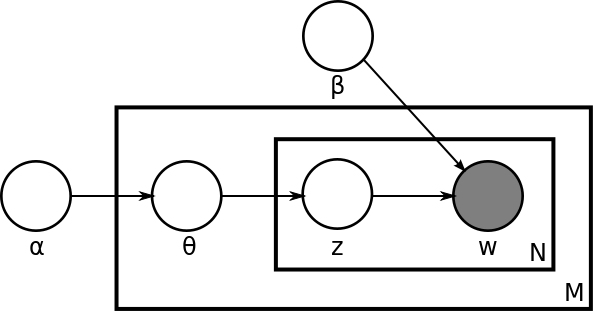
\includegraphics[width=15cm, height=6cm, keepaspectratio]{/Users/colehollant/Projects/sproj/resources/lda-not-verbose.png}
  
  \caption{Plate diagram for LDA \cite{593pxLat90:online}}
  \label{fig:ldaplate}
\end{figure}


Within the classic plate diagram for LDA (figure \ref{fig:ldaplate}), we have $M$ documents, $N$ topics, and an unlabelled vocabulary $V$. We take the topic distribution $\theta$, a $K$-dimensional random variable as drawn from a Dirichlet distribution, $\alpha$. On the other end, $\beta$ is a $K \times V$ matrix for a vocabulary of size $V$ that defines the word-topic probabilities. Arrows between nodes represent dependency, and $w$ is the sole darkened node as it is the only observed variable, all others are latent.

With probabilistic latent semantic indexing, an occurrence of a word is modeled as a sample from a topic mixture, leading to a probability distribution on a set of topics. Ng, Blei, and Jordan sought to extend this to account for document-level probabilities. Documents are mixtures with latent topics that are defined by a distribution of words.

With LDA, we are able to fix some number of topics, $K$, of which to determine; we can do this via collapsed Gibbs sampling. We begin with a random assignment of words in each document to topics $Z_{0\dots K}$ from a Dirichlet distribution as some initial document-topic representation and as some defined word-distribution for each topic.

From here, we fall into a training loop. We consider each document $d$, and each word $w$ within each document, we must compute $p(t | d)$ as well as $p(w | t)$ for each topic $t$. Then we will reassign $w$ to a topic, $t$, with probability $p(t | d) \cdot p(w | t)$, or the probability that $t$ has generated $w$. Note that the reassignment step assumes all word-topic distributions to be correct except for that of $w$. Once we reach convergence, or exhaust a defined number of epochs, we hope to see reasonable word-topic and document-topic distributions, which we can use to infer topic mixtures of documents.

Determining the probability of a topic given a word is an application of Bayes theorem:
$$p(t | w) = \frac{p(w | t)\cdot p(t)}{p(w)}$$

\noindent where we know the probability of a word (as informed by our corpus), the probability of a topic being chosen, and the probability of a word given a topic (as informed by the model state). Bear in mind, this has been glossed over as we did not focus on the implementation, for further reading, one should read Darling \cite{darlingl99:online}, or Blei et al. \cite{david_m._y._i._1970} \cite{TopicMod43:online}.

\subsection{Latent Dirichlet Allocation Scoring Model}
\vspace{12pt}
\subsubsection{\textbf{Building the model}}

For the LDA scoring model, we are to construct an LDA model and then determine some score from the output. We are using \texttt{gensim} for our implementation, and thus are almost exclusively concerned with determining the corpus to feed it. For this, we have grouped all entries in both the affect-intensity and senselevel lexicons by affect and gave all words by affect as our four seed documents.
$$\text{corpus} = \left\{\text{anger}, \text{fear}, \text{joy}, \text{sadness}\right\}\\\text{anger} = \left\{\text{word}\mid \text{word has affect score for angry}\right\}$$

\noindent This grouping was relatively painless, for affect intensity, we looked for non-zero scores in a given affect as criteria for membership, and we looked for affect existence within the senselevel lexicon; from here, we just combine them.

It is worth noting that this is an unusual means of gathering a corpus. Typically, a corpus is some large collection of documents, which would lend itself to repeated words with various frequencies throughout the documents. Our usage, on the other hand, holds that a word has a maximum document frequency of one. This then has implications on the model that uses things like term frequency inverse document frequency (tf-idf) \cite{david_m._y._i._1970} as a means of determining topic likelihood. With such strong limitations on intra-document frequency, uniqueness becomes more important. As a nicety for our model, we stem all tokens within our corpus. This maps words onto their root (i.e. $\left\{ \text{stem}, \text{stems}, \text{stemmed} \right\} \rightarrow \text{stem} $), and it allows for removing inconsistencies in the scoring of similar words. With stemming, all words sharing a root are given the same score, which is the average score of entries mapping to the stem. We also remove stop words from the tokens if present.

From here, building our model is as simple as passing our corpus and vocabulary along with some $K$ for number of topics and some number of epochs to gensim's \texttt{LdaModel} and save the model to disk. Note, we must save the model once and load it for all future use for the sake of consistency.

\subsubsection{\textbf{Using the model}}

In order to use the model, we ought to give our input the same treatment that our corpus was given. We will case-transform, filter by stop words, and stem the input strings. From here we loop over the inferred topic distribution in order of decreasing probability, and gather a few scores. For each topic with probability greater than a passed threshold, we gather: the topic probability, topic index, the $n$ topic keywords, and a few different means of scoring. We give four scores for each topic (and the net scores weighted by respective topic probabilities): the \texttt{input score} is the sum of the product of input token scores and their probability within the topic; the \texttt{topic score} is the sum of the product of vocabulary token scores and their probability within the topic; and there are two forms of \texttt{keyword} scores, one of which takes the topic keywords product with the normalized probability of the keywords, and the other takes the topic keywords product with the whole topic's probabilities.

\subsubsection{\textbf{LDA Model Endpoints}}

This also has a basic \texttt{GET} handler as a healthcheck. The \texttt{POST} handler here takes a float for the topic probability-threshold and an integer for the number of keywords to gather. There is an additional \texttt{GET} with a route parameter for topic number, should one want to observe the word probabilities for a given topic; this is not accessed by the frontend, but is accessible from \href{https://sproj.model.colehollant.com/lda/topic/1}{sproj.model.colehollant.com/lda/topic/\<topic-number\>}. One of the interesting pieces that arose from the translation from CLI to web server here was that \texttt{numpy}'s \texttt{float32} wasn't serializable; but as this is used within \texttt{gensim}'s model that we use, we have to provide a means of serialization which converts to \texttt{float64} \cite{Howtoser37:online}. This eases the process of tracking down instances of \texttt{float32}, and lets the \texttt{json} module handle this for us instead.

\subsection{LDA Model On Seeds}

It's worth considering the inferencing of the seed documents to see how they are scored. As each seed document was intended to represent a given affect-category, we would hope to see high scores in the corresponding category when fed the document. For this, we will look at the different net scores determined by feeding in each document with a $1\%$ probability threshold, gathering the top 100 keywords (scores will be rounded to 5 places).

\subsubsection{\textbf{Anger}}

\begin{table}[h!]
    \raggedright
    \begin{tabular}{|l|l|l|l|l|}
    \hline
    Category & Anger & Fear & Joy & Sadness \\\hline
    Input Score & \textbf{0.94886} & 0.76935 & 0.03475 & 0.67535 \\\hline
    Topic Score & 0.59074 & \textbf{0.59339} & 0.03516 & 0.53103 \\\hline
    Keywords by Keywords & \textbf{0.66098} & 0.65198 & 0.01993 & 0.58062 \\\hline
    Keywords by Topic & \textbf{0.25617} & 0.24547 & 0.00825 & 0.20950 \\\hline
    \end{tabular}
\end{table}

\subsubsection{\textbf{Fear}}

\begin{table}[h!]
    \raggedright
    \begin{tabular}{|l|l|l|l|l|}
    \hline
    Category & Anger & Fear & Joy & Sadness \\\hline
    Input Score & 0.65673 & \textbf{0.87143} & 0.01797 & 0.76317 \\\hline
    Topic Score & 0.51107 & 0.59343 & 0.04255 & \textbf{0.60067} \\\hline
    Keywords by Keywords & 0.58840 & 0.64486 & 0.03415 & \textbf{0.64810} \\\hline
    Keywords by Topic & 0.20910 & \textbf{0.22217} & 0.01214 & 0.21510 \\\hline
    \end{tabular}
\end{table}

\subsubsection{\textbf{Joy}}

\begin{table}[h!]
    \raggedright
    \begin{tabular}{|l|l|l|l|l|}
    \hline
    Category & Anger & Fear & Joy & Sadness \\\hline
    Input Score & 0.04641 & 0.06371 & \textbf{0.97432} & 0.07960 \\\hline
    Topic Score & 0.05247 & 0.07051 & \textbf{0.51985} & 0.06841 \\\hline
    Keywords by Keywords & 0.05356 & 0.07832 & \textbf{0.61078} & 0.08025 \\\hline
    Keywords by Topic & 0.01923 & 0.02722 & \textbf{0.20237} & 0.02747 \\\hline
    \end{tabular}
\end{table}

\subsubsection{\textbf{Sadness}}

\begin{table}[h!]
    \raggedright
    \begin{tabular}{|l|l|l|l|l|}
    \hline
    Category & Anger & Fear & Joy & Sadness \\\hline
    Input Score & 0.62026 & 0.80163 & 0.01106 & \textbf{0.99642} \\\hline
    Topic Score & 0.47046 & 0.60619 & 0.03291 & \textbf{0.66378} \\\hline
    Keywords by Keywords & 0.55249 & 0.64956 & 0.02865 & \textbf{0.70967} \\\hline
    Keywords by Topic & 0.18193 & 0.20938 & 0.00980 & \textbf{0.22397} \\\hline
    \end{tabular}
\end{table}

This makes intuitive sense. The input scores for each affect category are championed by their affect. The other scores are affected by the topic definition and keywords without direct scoring of the input, leading to greater fluctuation, although they tend to follow the trends of the input scores. We may notice the tendency of ``anger,'' ``fear,'' and ``sadness'' sharing similar scores that seem to oppose that of ``joy.'' This can be inferred to be a similarity between those emotions, but additional data may give further insight. We'll consider the mean Valence Arousal Dominance (VAD) scores for each document.

\subsubsection{\textbf{VAD By Category}}

\begin{table}[h!]
    \raggedright
    \begin{tabular}{|l|l|l|l|}
    \hline
        Category & Valence & Arousal & Dominance \\ \hline
        Anger & 0.25627 & 0.66386 & 0.46530 \\ \hline
        Fear & 0.28537 & 0.65718 & 0.47638 \\ \hline
        Joy & 0.7726 & 0.51821 & 0.59808 \\ \hline
        Sadness & 0.23668 & 0.58389 & 0.38429 \\ \hline
    \end{tabular}
\end{table}

Here we can see a tangible difference in valence scores between the group of ``anger,'' ``fear,'' and ``sadness'' having rather low mean valence scores, whereas ``joy'' has a rather high mean valence score. All the arousal and dominance scores across the affect categories have far less extreme values. We can use this as a means of understanding the uneven groupings of our affect categories as a latent bias regarding valence. This correlation also held for the most prevalent color associations across each document with ``anger'' and ``fear'' having ``black, red, gray;'' ``sadness'' having ``black, grey, red;'' and ``joy'' having ``white, yellow, pink'' as the top three most prevalent color associations.









\chapter{Frontend}

\section{Why make a frontend?}

There's a certain challenge to making your work accessible. Building and deploying a web application necessitates a different skill set than that required by the implementation of algorithms. There are layers added and layers complexified in shifting from a command line based program to a UI. A common practice of reading/writing from local files translates to managing some sort of data store, be it a proper database or some sort of browser storage like cookies, local storage, IndexedDB, or whatnot. We made a portal to accompany our APIs in order to have our work accessible to whoever may wish to use it regardless of their background in programming.

\subsection{Overview of our frontend}

Our webapp is a Single Page Application (SPA) built using VueJS \cite{Vuejs17:online}. Vue is one of big players in terms of frontend frameworks along with Facebook's ReactJS \cite{React-AJ42:online} and Google's Angular \cite{Angular31:online}, and is renowned for it's simplicity, scalability, and speed. We used the Vue CLI tool for development and building, although there is alternatively a library for the view layer via jsdeliver \cite{httpscdn6:online}. As such, we have largely kept to the structure of the scaffolding, keeping top level directories for assets, components, composables, and views. Composables were added later with the adoption of Vue's new composition API—in RFC (request for comments) at the time of use—which gives a fundamentally different way to interact with the Vue instance, giving a hook-oriented/function-based approach as opposed to the previous options API (an approach based off of certain properties in an object). Outside of Vue, we have several dependencies for the odd piece here and there, the largest part of the workflow would be tailwindcss \cite{Tailwind13:online}: a utility-based CSS framework. Tailwind ultimately gives a wide array of low-level utility classes that make for more concise CSS, and more flexible in-template stylings.

Our project is a SPA, although it has many views. Traditional websites may have several files that are served per URL, the rise of web applications led to a need for routers that mount and unmount components based on \texttt{window.location}. The Vue-Router takes an array of objects that specify path and may specify other aspects, including the component to mount, name, redirect location, and props. We strictly specified path, name, and component for our routes, and we left the router in hash mode to save on some server config for associated with history mode; we have routes for the home page, the thesaurus, the models, writing, documentation, and presentations. As per the likeness in characteristics, we will use ``routes'' and ``pages'' interchangably.

The home page simply serves as a hub to link to all pages as well as the repository on GitHub, as the main navbar does not span all routes. The thesaurus page gives an input box to query the thesaurus and senselevel collections, and displays synonyms and antonyms by part of speech as well as sense associations by word-sense including synonyms shared between the sense words and the queried word. The model page offers interaction with each of our models; the model is selected through a dropdown menu, and the associated controls are displayed (a textbox, various inputs such as sliders and toggles for targeting the endpoint's parameters, and a submit button); each model has a unique results section. The writing section is very simply an online version of this paper rendered to HTML and injected. The documentation page is a custom renderer for our Postman collection \cite{PostmanT86:online}. Postman is the HTTP client we used for development to organize requests and inject variables for things like staging; it also allows for exporting your collection as JSON, which we are using to inform our documentation page. The presentation route holds our HTML presentation rendering which allows for ease of access and navigation.

\subsection{Configuration}

There's not too much configuration to be done here as per the fairly minimal frontend and the niceties that Node has to offer. There are a few config files to edit to get tailwind integrated and to add our customizations to it, and there is some tinkering with webpack \cite{webpack35:online} to add a loader to import \texttt{.txt} files as strings. We set \texttt{NODE\_ENV} within our start scripts to be able to target different URI's for our APIs.

\section{Creating our Component Library}

Various frameworks take different approaches to organizing the HTML, CSS, and Javascript that make up each component. Some frameworks, like Angular, tend to keep separate files for each piece of the component, whereas frameworks like Vue opt for single file components (SFC). This is simply an organizational difference, and each approach has pros and cons. We need various components to build our frontend, from basic UI components like text inputs and sliders to page components that are associated with each route. As per the options API, each component may take a set of \textit{props}, which specifies data to be passed to them from the parent; this follows Vue's one-way data flow principle—should data have to be passed to a parent, we do so by emitting events and attaching a listener to the parent.

\subsection{Different Kinds of Components}

There are multiple ways to write components within Vue. There are different ways to target the template; one of which is to write all of the markup in HTML with directives and bindings like \texttt{v-if}, \texttt{v-for}, \texttt{v-bind}, \texttt{v-on}, and other way is through the render function. The render function is what is used underneath the hood; Vue compiles the markup templates to a render function that creates a VNode (virtual node), as Vue is based on the virtual DOM. The render function taking some parameter to specify tag or component options, an object that translates to element attributes, and a list of children. There is also a distinction between functional and full-featured components; functional components do not manage their own state, watch state, nor have lifecycle hooks, and thus do not need the same reactivity that full-featured components require. Below is an example of the same UI represented as a render function and as a template for the sake of comparison:
\begin{figure}
\footnotesize{
\begin{lstlisting}[language=C]
render(h, {props, listeners}) {
  const hasResults = (obj) => {
    for(let key of Object.keys(obj)){
      if(obj[key].length > 0) return true;
    }
    return false
  }
  let entry = props.entry;
  return h("div", { staticClass: "my-12" }, [
    h("div", {
        staticClass: "thesaurus--results-box",
      }, [
      Object.keys(entry).map(key => {
        return hasResults(entry[key]) ? h("div", {}, [
          h("h2", {
            staticClass: "thesaurus--category",
            domProps: { "innerHTML": key },
          }),
          h("div", {
            staticClass: "thesaurus--pos__wrapper"
          }, Object.keys(entry[key]).map(pos => {
            if(entry[key][pos].length > 0) {
              return h("div", { staticClass: "mx-4 md:mx-8"}, [
                h("h3", { staticClass: "thesaurus--pos" }, pos),
                h("ul", { "class": "thesaurus--entry__wrapper" }, 
                  entry[key][pos].map(word => {
                    return h("li", {
                      attrs: { tabindex: 0 },
                      staticClass: "thesaurus--entry",
                      domProps: { "innerHTML": word },
                      on: {
                        keydown: (e) => {
                          if(e.key === 'Enter' || e.key === ' ') {
                            const emit_event = listeners.event_from_child;
                            emit_event(word);
                          }
                        },
                        click: () => {
                          const emit_event = listeners.event_from_child;
                          emit_event(word);
                        }
                      }
                    })
                  })
                )
              ])
            }
          }))
        ]) : null
      })
      ] 
    )
  ])
}
\end{lstlisting}
}
\caption{Component markup through render function}
\end{figure}
\begin{figure}
\footnotesize{
\begin{lstlisting}[language=XML]
<template functional>
<div class="thesaurus--results-box">
  <div 
    v-for="(key, i) in Object.keys(props.entry)" 
    :key="[key, i].join('-')"
  >
    <div v-if="Object.entries(props.entry[key]).map(([k, v]) => v.length > 0).reduce((a, c) => (a || c))">
      <h2 class="thesaurus--category">
        {{ key }}
      </h2>
      <div class="thesaurus--pos__wrapper">
        <div 
          v-for="(pos, j) in Object.keys(props.entry[key])" 
          :key="[pos, props.entry.key, j].join('-')"
        >
          <div 
            v-if="props.entry[key][pos].length > 0" 
            class="mx-4 md:mx-8"
          >
            <h3 class="thesaurus--pos">
              {{ pos }}
            </h3>
            <ul class="thesaurus--entry__wrapper">
              <li 
                class="thesaurus--entry" 
                v-for="(word, k) in props.entry[key][pos]" 
                :key="[pos, props.entry.key, word, k].join('-')" 
                v-on:keydown.enter="() => listeners.event_from_child(word)" 
                v-on:keydown.space="() => listeners.event_from_child(word)" 
                v-on:click="() => listeners.event_from_child(word)" 
                tabindex="0"
              >
                {{word}}
              </li>
            </ul>
          </div>
        </div>
      </div>
    </div>
  </div>
</div>
</template>
\end{lstlisting}
}
\caption{Component markup through template}
\label{fig:template}
\end{figure}

Ultimately the render function provides greater flexibility with all of Javascript at your disposal rather than relying on the tools provided by Vue through directives. Writing raw render functions is a process somewhere between writing JSX (which render functions support as an alternative through a Babel plugin), and writing Javascript without a framework to manipulate the DOM.

\subsection{Our Components}

We have all basic UI components within a directory with the following components: \texttt{InfoHover}, \texttt{Loading}, \texttt{ProgressBar} \texttt{Slider}, \texttt{TextInput}, \texttt{Toggle}, \texttt{WordList}. \texttt{InfoHover} provides an info icon with a child conditionally rendered on hover or on click via a \texttt{slot}; we have a prop for \texttt{size} that controls the width and height of the icon-button, as \texttt{size} can only take certain values, we add a validator to ensure that valid values are used. \texttt{Loading} is a simple loading spinner that is displayed while a request is being processed, we do this with partial border coloring and infinite-duration CSS animations—this is a component that makes a clear case to be a functional component, as it doesn't even need it's own Javascript to function. \texttt{ProgressBar} gives a rectangle colored proportionally to the \texttt{value} prop and with a color mapped to by the \texttt{color} prop; \texttt{color} also has a validator attached. \texttt{Slider} wraps the default \texttt{type=``range''} input, taking care of data binding, styling, and providing a slot for a label; there are props for \texttt{min}, \texttt{max}, \texttt{step}, and \texttt{value}. \texttt{TextInput} is similar to \texttt{Slider} in that it wraps the default \texttt{type=``range | X''} input, handles data binding and styling, and has props for \texttt{value} and \texttt{error} which is a string that affects style and adds a message to the DOM. \texttt{Toggle} is a wrapper for the default \texttt{type=``checkbox''} input that overhauls the styling in order to target the feel of a switch rather than a checkbox; this only takes a prop for \texttt{value}. \texttt{WordList} eases the process of rendering each word from an array, simply looping over the items in it's \texttt{value} prop and displaying them in order. These are all basic UI building blocks that are used throughout the application, and largely serve to bind date or display pieces of information passed to them.

There are a few other components across the application that don't quite fit within the basic UI group nor the documentation group. These include \texttt{ScoreBars}, \texttt{GroupScores}, \texttt{NetScores}, \texttt{Navbar}, \texttt{SenseLevelResult}, \texttt{ThesaurusResult}, and \texttt{ThesaurusEntry}. \texttt{ScoreBars} displays a group of labelled \texttt{ProgressBar}s or a label signifying that each value was zero; there are props for \texttt{name}, \texttt{size}, and \texttt{value}. \texttt{GroupScores} renders a series of \texttt{ScoreBars} for the output of each topic in the LDA model, and only takes a \texttt{value} prop. \texttt{NetScores} operates similarly to \texttt{GroupScores}, but ignores trying to render some properties that do not exist. \texttt{Navbar} only displays a group of \texttt{router-link}s. \texttt{SenseLevelResult} handles the senselevel rendering; it must make a request to our API for the current word and parse the response, finding common synonyms, and organizing by sense. \texttt{ThesaurusResult} takes the response from the thesaurus endpoint and renders the result by synonym/antonym and part of speech; this was a place we wrote our own render function. \texttt{ThesaurusEntry} is a layout component that gives a text input for the current word and renders the \texttt{SenseLevelResult} and \texttt{ThesaurusResult} components upon submission.

\subsection{Creating Our Documentation Renderer}

A large part of using components is to break down monolithic markup into readable and maintainable chunks under the assumption that fifty small files with a narrow focus are easier to grasp than a handful of huge files responsible for a wide range of behavior. The other is to cut down on the copy-pasting of similar markup that will be used multiple times. Both usages appear within our documentation renderer.

We have a layout component, \texttt{DocRenderer}, that receives an object representing the JSON from the documentation and sends appropriate data to its children based off of the current selected folder. \texttt{DocRenderer} provides a navigation bar with a link to \texttt{/home}, buttons for each folder of requests, and buttons for each request within the selected folder. We make use of gsap's \cite{GSAPGree71:online} \texttt{ScrollToPlugin} to scroll to the correct page offset once a user selects a request. We pass the selected folder to our \texttt{Folder} component, which displays a header with a name and description, and mounts a series of \texttt{DocRequest} components for each request within the folder; this uses markdown-it \cite{markdown14:online} as a markdown rendering engine for the description. \texttt{DocRequest} is a component responsible for rendering a single request's information; it displays name, HTTP method, url, description, request headers, request body, and response, the latter three being abstracted to components. \texttt{Headers} renders a table of accepted headers for the current request; \texttt{Body} and \texttt{Response} render the request body and response as preformatted JSON—prettified by re-parsing and stringifying—with the additional status code section for the \texttt{Response} to render. Put together with example responses and targeted requests through Postman, we arrive at an intuitive documentation portal for our API in place of a 3.3M JSON document.

\section{Consuming the composition API}

The Vue Composition API provides a means to the level of abstraction achievable through components. This serves not necessarily to replace the options API, but to compliment it, and to give greater access to the underlying APIs of Vue. It's usage within this project is limited to that of \texttt{useModel}, as it has only come out over the course of this project. While it is limited in its use across our frontend, \texttt{useModel} manages to be used by each of our four model components. \texttt{useModel} serves as a testament to the use-case of the composition API as we are able to abstract almost all logic from the model components. Rather than binding reactive data via entries within the \texttt{data} property, we are given \texttt{ref} and \texttt{reactive} which can be used \textit{largely interchangeably} although \texttt{ref} is more-so for Javascript primitives and \texttt{reactive} is for objects (that is \texttt{ref} calls \texttt{reactive} when given an object and \texttt{reactive} cannot accept primitives), and values are exposed to the template by returning from the \texttt{setup} function.

As such, each model component has various reactive state corresponding to the inputs—a \texttt{ref} for the text input, the probability of changing a word, whether to ignore stopwords, etc—and state returned by the model targeted within \texttt{useModel}. Each model hook exported by \texttt{useModel} calls the \texttt{useModel} function, passing the appropriate endpoint; this is a higher order function wrapping \texttt{responseState}—a \texttt{reactive} object with properties relevant to rendering an HTTP response—and a function called \texttt{postData} that wraps \texttt{window.fetch} to deal with the repeated logic across requests for injecting endpoints and binding data to \texttt{responseState}. This allows for a large reduction in repeated logic across the four model components, in that each component only needs to call \texttt{postData} with the request body.

\section{Making things pretty}

Much of the frontend is complex purely for the reason of aesthetics. Out of the box, without any CSS, we get a functional, responsive website; it will be black text left justified on a white background, and it will look as though the text content of a website was copied and pasted into a Word document. This is to say, it will work, although it may be significantly harder and less enjoyable to use. User interfaces and user experience (UI/UX) play a large role in web development with UX informing how a site should work and UI informing how it should work.

We have already seen a decent amount of this with our base UI components, that often served to override the default HTML inputs. Among the simpler examples would be our \texttt{TextInput} component; here we specify that the text should align left and that the element should take the full width of the parent on the wrapper element, and we pass styles to the \texttt{input} element. We apply the classes \texttt{[w-full px-2 font-normal rounded border-2 border-primary-50 text-primary-10 appearance-none]} which are generated by tailwind and translates to:
\begin{figure}[h!]
\begin{lstlisting}[language=XML]
{
  width: 100%;
  padding-left: 0.5rem; 
  padding-right: 0.5rem;
  font-weight: 400;
  border-radius: 0.25rem;
  border: 2px solid var(--primary-50);
  color: var(--primary-10);
  appearance: none;
}
\end{lstlisting}
\caption{CSS properties and values targeted by tailwind's \texttt{w-full px-2 font-normal rounded border-2 border-primary-50 text-primary-10 appearance-none}}
\end{figure}

We also add some variants to the \texttt{input} element. We add focus styles, placeholder styles, and dark mode variants. The associated error message element features orange text, a heavier font-weight, a smaller text size, and a different text alignment to set it off from the styles of the \texttt{input} and to signify that something has gone wrong.

Often, the main pieces of markup are the layout containers and the content elements. The layout container is responsible for the positioning of its children in a general sense: we may have a \texttt{display: flex; flex-direction: row} container that uses \texttt{justify-content: between; align-items: baseline} which places its children evenly across its full extent of the x-axis and are set on the y-axis such that their baselines are even; a layout container with \texttt{display: grid; grid-gap: 1rem} would display its children in a single column with 1rem of space between each item. Content elements tend to set properties like the typography, margin, etc that only affect the element itself.

CSS is a large, tricky, beautiful language. Despite the power behind it, there's little to discuss without getting far into specifics regarding my design choices. Rather than get into why some places have 18pt font and others have 14pt and other similar decisions, I will point to w3 schools \cite{CSSTutor62:online} to learn more on CSS, and leave a line of Javascript that you can put in your browser's developer console to disable the CSS stylesheets for the page you are on (only until you reload):

\begin{lstlisting}[language=C]
for (const s of document.styleSheets) s.disabled = true
\end{lstlisting}

\section{Making things accessible}

Where beautification may not be the most important aspect to discuss, accessibility absolutely warrants a nod. Accessibility is something often overlooked in websites, especially among junior developers; as a junior developer myself, I am not an expert, but there are several easy steps you can take to improve the accessibility of your site.

In creating something navigable by keyboard, the user will be traversing between elements largely through arrow keys and the tab key. When an element has focus, there is some sort of ring around it, for example \texttt{outline: 5px auto -webkit-focus-ring-color} this stands out to signify which element has focus. This focus ring is not the prettiest in terms of UI, despite being functional, and so as to avoid the focus ring rising when things like buttons are clicked (or other elements that receive focus without dismissing on click), it is unfortunately common to see many elements with \texttt{selector:focus { outline: none }} which leaves keyboard users unable to properly determine what element has focus. In order to achieve a pretty UI while considering accessibility, we create specific focus styles for relevant focusable elements; this can come in the form of tailwind's \texttt{shadow-outline} that applies a solid blue box-shadow around the element (as box-shadow respects border-radius, but outline does not), an underline (although this is rarely sufficient), or changes in background/text/border color.

There are several other key aspects to accessibility; one of which is the use of screen readers. This is something harder to target if you aren't specifically trying to, as it often has no impact for those that are seeing, and many people either do not have a screen reader or are not proficient in using it. That being said, there are several easy pieces that can be addressed to improve the experience of using your site via screen reader: using semantic HTML where applicable rather than creating and styling generic elements (\texttt{div}s and \texttt{span}s) gives more insight as to what the element is; using appropriate headings when applicable helps with navigation; and proper labels for inputs gives insight into the functionality of controls. The latter piece, with labels, is something noteworthy as it is still common to see inputs use placeholder text in place of labels; this may sound reasonable, but screen readers need a label to read as a prompt once there is focus. There \textit{is} a practice, which is commendable, of providing text nodes that are only accessible via screen reader (essentially creating elements that are present but invisible), although providing a screen reader only label may not even be enough! Chrome's auto translation has skipped over translating attributes (including placeholder), which leaves an untranslated label; even beyond this there are accessibility issues at stake with recall such that a user may lose track of the label for an input if it is a placeholder that disappears once it receives input; there are issues with color contrast ratios of placeholder text, and so on.

On the subject of \texttt{div}s in place of semantic HTML, there is a level of difficulty in replicating certain default behavior of existing tags. In our earlier example of render functions versus templates \ref{fig:template}, there was a list item being used as a button for each word. This is acceptable, although for it to \textit{work} as a button, there are several pieces we must add for a function to be called replicating the \texttt{onclick} attribute of the button, we must add a click event listener and a keydown event listener that calls the function hitting the spacebar or return key; in order to take focus via tab, we must provide \texttt{tabindex=``0''}.

Contrast ratios are one of the most common problems for visually impaired users. There is a formula from the Web Content Accessibility Guidelines (WCAG) \cite{WebConte88:online} that determines contrast score and ratio, although there are certain aspects of contrast like hue difference that are largely ignored, as well as CSS properties that contribute to contrast—like shadows. Regardless of its flaws, it serves as a reasonable heuristic for accessible typography. Some browsers are able to provide contrast scores from within the developer tools, which helps a developer to determine if their site is meeting minimum contrast ratios.

In terms of browser support for assisting in targeting accessibility issues, there are certain developer features browsers may have to audit a webpage's accessibility features. Chrome does this via lighthouse \cite{Lighthou16:online}, which again has politics attached in that it is run by Google who targets certain things that make it easier to serve ads, etc. Disclaimer aside, it is a powerful, helpful tool that can automate some (not all) of accessibility checking, checking things including:

\begin{lstlisting}[language=C]
- [aria-*] attributes match their roles
- [aria-*] attributes have valid values
- [aria-*] attributes are valid and not misspelled
- Buttons have an accessible name
- The page contains a heading, skip link, or landmark region
- Background and foreground colors have a sufficient contrast ratio
- Document has a <title> element
- [id] attributes on the page are unique
- <html> element has a [lang] attribute
- <html> element has a valid value for its [lang] attribute
- Form elements have associated labels
- Links have a discernible name
- Lists contain only <li> elements and script supporting elements (<script> and - <template>).
- List items (<li>) are contained within <ul> or <ol> parent elements
- [user-scalable="no"] is not used in the <meta name="viewport"> element and the - [maximum-scale] attribute is not less than 5.
- No element has a [tabindex] value greater than 0
\end{lstlisting}

Our frontend is not perfect on every page even by the lighthouse audits—it reports that the documentation page is missing a title page, and there is insufficient contrast on the request method badge, leading to a score of 91/100. It is a per-page audit, and gives clear feedback on what must be done to address the concerns, which is a wonderful nicety in terms of developer experience, and helps to keep people aware of serious concerns with their websites.








\chapter{Experiment}

\section{Experimental Design}

\textit{Note: All experimentation was conducted with IRB approval.}

We conducted a survey to determine a baseline of human scores for passages by affect. This allows us to assess the performance of our scoring models, such that a model is better than another if it is closer to human scores. We had to undergo this experiment as there is a lack of labelled data in this form. There were two versions of the survey; both had the same first twelve passages, and a different set of the latter twelve passages. The first twelve passages were gathered by a sentence generator and served as unaltered text. The second set of twelve passages was gathered by feeding the first twelve through one of our replacement models; one version of the survey had all passages go through the arbitrary replacement model, and the other had all passages go through the targeted replacement model. For each passage, we asked the participants to give a score from one to ten in each of the following categories: how natural the passage sounded, how angry the passage sounded, how sad the passage sounded, how joyful the passage sounded, and how fearful the passage sounded.

This was conducted over the internet via Google Forms. As Forms does not support A/B testing, we embedded the surveys in a webpage using a \href{https://github.com/colehollant/quarantine-js}{microframework I built} to programmatically provide one of the two versions with equal probability. We received 30 responses across the two surveys, with an even split of 15 responses for each version. This is a rather small sample size to draw generalizations on humans, but is adequate to gather the labelled data that we desire. There are core issues present, in that the participants were almost exclusively college-educated and are mostly white. Ideally, we would have a much larger sample size of at least several hundred that better represents the United States' population.

\subsection{Stats}

% Also, you need a Stats section in the methods, describing each of the tests you did and why they are appropriate 
We conducted an independent sample t test on the control results for each category (scores for natural, anger, sadness, joy, fear) to gain insight on the difference between the two groups. Each category has a null hypothesis of the two groups having equal means; each category has the same 12 prompts (given below), and we run the t test on each question of each prompt. We will also run a series of relative-error tests, assuming that the human scores are the expected scores. This allows us to determine which scoring algorithm is most appropriate.

\subsubsection{\textbf{Prompts}}
\begin{tabular}{|l|}
  \hline
    question \\ \hline
    \texttt{01.}\hspace{8pt} When motorists sped in and out of traffic,\\\hspace{24pt} all she could think of was those in need of a transplant. \\ \hline
    \texttt{02.}\hspace{8pt} He drank life before spitting it out. \\ \hline
    \texttt{03.}\hspace{8pt} The toy brought back fond memories of being lost in the rain forest. \\ \hline
    \texttt{04.}\hspace{8pt} Italy is my favorite country; in fact, I plan to spend two weeks there next year. \\ \hline
    \texttt{05.}\hspace{8pt} The blinking lights of the antenna tower came into focus just as I heard a loud snap. \\ \hline
    \texttt{06.}\hspace{8pt} I love bacon, beer, birds, and baboons. \\ \hline
    \texttt{07.}\hspace{8pt} She saw the brake lights, but not in time. \\ \hline
    \texttt{08.}\hspace{8pt} They say that dogs are man's best friend, \\\hspace{24pt} but this cat was setting out to sabotage that theory. \\ \hline
    \texttt{09.}\hspace{8pt} The tart lemonade quenched her thirst, but not her longing. \\ \hline
    \texttt{10.}\hspace{8pt} He was surprised that his immense laziness was inspirational to others. \\ \hline
    \texttt{11.}\hspace{8pt} They got there early, and they got really good seats. \\ \hline
    \texttt{12.}\hspace{8pt} You can't compare apples and oranges, but what about bananas and plantains? \\ \hline
  \end{tabular}
\vspace{16pt}

\section{Results}

\subsection{Comparison of groups}

In the independent sample t tests to compare the two groups, the ``natural'' category had one out of twelve p values below our $\alpha = 0.05$, thus in all other cases we fail to reject the null hypothesis—we are unable to conclude that the two groups are significantly different. Similarly, the ``anger'' category had one out of twelve, ``sadness'' had two out of twelve, ``joy'' had one out of twelve, and ``fear'' had two out of twelve p values less than $\alpha = 0.05$.

\subsubsection{\textbf{Natural Scores}}

\begin{tabular}{|l|l|l|l|l|l|l|l|}
\hline
    question & p value & mean difference & upper CI & lower CI & df & Cohen's d & effect size \\ \hline
    1. & 0.48079 & 0.57143 & 1.28675 & -0.14389 & 26 & 0.27037 & small \\ \hline
    2. & 0.94782 & 0.07143 & 0.13751 & 0.00535 & 26 & 0.02498 & small \\ \hline
    3. & 0.34479 & 0.71429 & 1.67654 & -0.24796 & 26 & 0.3637 & medium  \\ \hline
    4. & 0.72381 & 0.28571 & 0.64294 & -0.07151 & 26 & 0.13502 & small \\ \hline
    5. & 0.49097 & -0.5 & -1.19866 & 0.19866 & 26 & -0.26407 & small  \\ \hline
    6. & 0.71533 & 0.28571 & 0.65443 & -0.083 & 26 & 0.13936 & small \\ \hline
    7. & 0.50865 & -0.42857 & -1.09875 & 0.2416 & 26 & -0.2533 & small \\ \hline
    8. & 0.37381 & -0.57143 & -1.47636 & 0.3335 & 26 & -0.34203 & small \\ \hline
    9. & 0.42139 & -0.78571 & -1.60264 & 0.03122 & 26 & -0.30877 & small \\ \hline
    10. & 0.70986 & 0.35714 & 0.73329 & -0.01901 & 26 & 0.14217 & small \\ \hline
    11. & \textbf{0.03027} & 1.57143 & 3.86317 & -0.72031 & 26 & 0.8662 & large \\ \hline
    12. & 0.30227 & 0.85714 & 1.90961 & -0.19533 & 26 & 0.3978 & medium \\ \hline
\end{tabular}
\vspace{16pt}

\subsubsection{\textbf{Anger Scores}}

\begin{tabular}{|l|l|l|l|l|l|l|l|}
\hline
    question & p value & mean difference & upper CI & lower CI & df & Cohen's d & effect size  \\ \hline
    1. & 0.14972 & 1.21429 & 2.69871 & -0.27014 & 26 & 0.56106 & medium \\ \hline
    2. & 0.07658 & -1.57143 & -3.41563 & 0.27277 & 26 & -0.69704 & small \\ \hline
    3. & 0.65964 & -0.14286 & -0.58836 & 0.30265 & 26 & -0.16838 & small \\ \hline
    4. & 0.45892 & -0.14286 & -0.89467 & 0.60895 & 26 & -0.28416 & small \\ \hline
    5. & 0.13268 & -0.64286 & -2.19515 & 0.90944 & 26 & -0.58671 & small \\ \hline
    6. & 0.06944 & -0.28571 & -2.17944 & 1.60801 & 26 & -0.71576 & small \\ \hline
    7. & 0.8948 & -0.07143 & -0.20497 & 0.06211 & 26 & -0.05047 & small \\ \hline
    8. & 0.45384 & -0.64286 & -1.40329 & 0.11757 & 26 & -0.28742 & small \\ \hline
    9. & 0.53799 & -0.28571 & -0.90982 & 0.3384 & 26 & -0.23589 & small \\ \hline
    10. & 0.18126 & -0.42857 & -1.80229 & 0.94514 & 26 & -0.51922 & small \\ \hline
    11. & 0.14574 & -0.71429 & -2.214 & 0.78543 & 26 & -0.56684 & small \\ \hline
    12. & \textbf{0.04879} & -0.85714 & -2.9245 & 1.21022 & 26 & -0.78139 & small \\ \hline
\end{tabular}
\vspace{16pt}

\subsubsection{\textbf{Sadness Scores}}

\begin{tabular}{|l|l|l|l|l|l|l|l|}
\hline
    question & p value & mean difference & upper CI & lower CI & df & Cohen's d & effect size  \\ \hline
    1. & 0.45453 & -0.5 & -1.25926 & 0.25926 & 26 & -0.28697 & small \\ \hline
    2. & 0.66341 & -0.35714 & -0.79737 & 0.08308 & 26 & -0.16639 & small  \\ \hline
    3. & 0.05728 & -1.78571 & -3.77509 & 0.20366 & 26 & -0.75191 & small  \\ \hline
    4. & 0.14936 & -0.21429 & -1.70007 & 1.2715 & 26 & -0.56157 & small \\ \hline
    5. & 0.68706 & 0.21429 & 0.62166 & -0.19309 & 26 & 0.15397 & small  \\ \hline
    6. & 0.7837 & -0.07143 & -0.34878 & 0.20592 & 26 & -0.10483 & small \\ \hline
    7. & 0.92345 & 0.07143 & 0.16845 & -0.02559 & 26 & 0.03667 & small \\ \hline
    8. & 0.06638 & -0.71429 & -2.63061 & 1.20204 & 26 & -0.7243 & small \\ \hline
    9. & 0.08258 & -1.28571 & -3.09128 & 0.51985 & 26 & -0.68244 & small \\ \hline
    10. & 1.0 & 0.0 & 0.0 & 0.0 & 26 & 0.0 & small  \\ \hline
    11. & \textbf{0.03373} & -0.78571 & -3.02749 & 1.45606 & 26 & -0.84731 & small \\ \hline
    12. & \textbf{0.03594} & -0.57143 & -2.78369 & 1.64084 & 26 & -0.83616 & small \\ \hline
\end{tabular}
\vspace{16pt}

\subsubsection{\textbf{Joy Scores}}

\begin{tabular}{|l|l|l|l|l|l|l|l|}
\hline
    question & p value & mean difference & upper CI & lower CI & df & Cohen's d & effect size  \\ \hline
    1. & 0.15908 & -0.64286 & -2.09261 & 0.8069 & 26 & -0.54796 & small \\ \hline
    2. & 0.91834 & 0.07143 & 0.17495 & -0.0321 & 26 & 0.03913 & small  \\ \hline
    3. & 0.71771 & -0.35714 & -0.72263 & 0.00834 & 26 & -0.13814 & small  \\ \hline
    4. & 0.73313 & -0.21429 & -0.55893 & 0.13036 & 26 & -0.13026 & small \\ \hline
    5. & 0.81512 & 0.07143 & 0.30764 & -0.16478 & 26 & 0.08928 & small  \\ \hline
    6. & 0.86097 & -0.14286 & -0.31974 & 0.03403 & 26 & -0.06686 & small \\ \hline
    7. & \textbf{0.03103} & -0.28571 & -2.56607 & 1.99464 & 26 & -0.86189 & small \\ \hline
    8. & 0.57205 & 0.5 & 1.07228 & -0.07228 & 26 & 0.2163 & small \\ \hline
    9. & 0.06454 & 1.07143 & 3.00174 & -0.85889 & 26 & 0.72959 & large \\ \hline
    10. & 0.42582 & -0.71429 & -1.52335 & 0.09478 & 26 & -0.3058 & small  \\ \hline
    11. & 0.93493 & -0.07143 & -0.15386 & 0.01101 & 26 & -0.03116 & small \\ \hline
    12. & 0.52145 & 0.64286 & 1.29277 & -0.00705 & 26 & 0.24564 & small \\ \hline
\end{tabular}
\vspace{16pt}

\subsubsection{\textbf{Fear Scores}}

\begin{tabular}{|l|l|l|l|l|l|l|l|}
\hline
    question & p value & mean difference & upper CI & lower CI & df & Cohen's d & effect size  \\ \hline
    1. & 0.64988 & 0.35714 & 0.81638 & -0.1021 & 26 & 0.17358 & small \\ \hline
    2. & 0.7244 & 0.21429 & 0.57071 & -0.14214 & 26 & 0.13471 & small  \\ \hline
    3. & 0.75466 & 0.21429 & 0.53011 & -0.10154 & 26 & 0.11937 & small  \\ \hline
    4. & \textbf{0.03103} & -0.28571 & -2.56607 & 1.99464 & 26 & -0.86189 & small \\ \hline
    5. & 0.325 & -0.85714 & -1.86036 & 0.14608 & 26 & -0.37918 & small  \\ \hline
    6. & 0.13199 & -0.28571 & -1.8409 & 1.26947 & 26 & -0.58781 & small \\ \hline
    7. & 0.10962 & -1.5 & -3.15662 & 0.15662 & 26 & -0.62614 & small \\ \hline
    8. & 0.86424 & -0.14286 & -0.31553 & 0.02982 & 26 & -0.06526 & small \\ \hline
    9. & 0.36909 & -0.35714 & -1.27119 & 0.5569 & 26 & -0.34548 & small \\ \hline
    10. & 0.61713 & -0.21429 & -0.72027 & 0.2917 & 26 & -0.19124 & small  \\ \hline
    11. & \textbf{0.02071} & -0.5 & -2.96306 & 1.96306 & 26 & -0.93095 & small \\ \hline
    12. & 0.21367 & -0.28571 & -1.56047 & 0.98904 & 26 & -0.48181 & small \\ \hline
\end{tabular}
\vspace{16pt}

\subsection{Error Analysis}

Then, we chose a subset of scoring metrics (raw score, and LDA net scores for input and topic) to compare to the real scores determined by our participants. We will use relative error as a means of analysis. Given the human scores as the expected scores, relative error serves to give a measure on how a model performs. We will look at relative error averaged by category, and then subdivided by target and group.

\subsubsection{\textbf{LDA Input Score Error}}

\begin{tabular}{|l|l|l|l|l|l|}
\hline
    anger error & sadness error & joy error & fear error & mean error & std dev \\ \hline
    -0.85802 & -0.76072 & -0.70641 & -0.79792 & -0.78077 & 0.055211 \\ \hline
\end{tabular}
\vspace{16pt}

\subsubsection{\textbf{LDA Topic Score Error}}

\begin{tabular}{|l|l|l|l|l|l|}
\hline
    anger error & sadness error & joy error & fear error & mean error & std dev \\ \hline
    -0.53525 & -0.46815 & -0.36493 & -0.47174 & -0.46002 & 0.061043 \\ \hline
\end{tabular}
\vspace{16pt}

\subsubsection{\textbf{Raw Score Error}}
\begin{tabular}{|l|l|l|l|l|l|}
\hline
    anger error & sadness error & joy error & fear error & mean error & std dev \\ \hline
    -0.85647 & -0.85213 & -0.85312 & -0.8497 & -0.85286 & 0.002430 \\ \hline
\end{tabular}
\vspace{16pt}

We can see that the LDA net scores for topic has the least average error across the board, followed by the LDA input scores, with the raw score trailing at the end. This suggests that the LDA topic score may be the most appropriate scoring model that we offer, although it has the highest variance among error scores. We can further look at our results by group and affect-target. Note that the ``group'' is either ``neutral'' for the unaltered sentences, ``control'' for sentences that went through arbitrary replacement, or ``experimental'' for sentences that went through targeted replacement; for the ``experimental'' group, we note the affect-target.

\subsubsection{\textbf{LDA Input Score Error}}

\begin{tabular}{|l|l|l|l|l|l|l|l|}
\hline
    group & target & anger err & sadness err & joy err & fear err & mean $|\text{err}|$ & std dev \\ \hline
    neutral &  & -0.96974 & -0.68386 & -0.84701 & -0.77157 & 0.81804 & 0.12113 \\ \hline
    control &  & -0.95562 & -0.95015 & -0.97787 & -0.79765 & 0.92032 & 0.08266 \\ \hline
    experimental & anger & -0.43843 & -0.48738 & -0.20712 & -0.98126 & 0.52855 & 0.32562 \\ \hline
    experimental & sadness & -0.56263 & 0.03343 & 0.67848 & -0.69709 & 0.49291 & 0.31204 \\ \hline
    experimental & joy & -1.0 & -1.0 & -0.39131 & -0.47553 & 0.71671 & 0.32892 \\ \hline
    experimental & fear & -0.79571 & -0.94346 & -0.89708 & -0.9416 & 0.89446 & 0.06924 \\ \hline
\end{tabular}
\vspace{16pt}

Here, we see that the LDA input scoring has rather high error with the unaltered (neutral) and random-replacement (control) scores ($>80\%$), and a mix of high and low error among the the targeted replacement scores. We see high average error within the sentences with a target of ``fear'' and ``joy'' ($89\% \text{ and } 72\%$ respectively), with lower mean error for sentences targeting ``anger'' and ``sadness'' ($53\% \text{ and } 49\%$ respectively).

\subsubsection{\textbf{LDA Topic Score Error}}

\begin{tabular}{|l|l|l|l|l|l|l|l|l|}
\hline
    group & target & anger err & sadness err & joy err & fear err & mean $|\text{err}|$ & std dev  \\ \hline
    neutral &  & -0.51351 & -0.65078 & -0.49961 & -0.39885 & 0.51569 & 0.10354  \\ \hline
    control &  & -0.67275 & -0.45844 & -0.48453 & -0.49215 & 0.52697 & 0.09826  \\ \hline
    experimental & anger & -0.0917 & 0.13595 & 0.41926 & -0.81972 & 0.36666 & 0.33509  \\ \hline
    experimental & sadness & -0.67467 & -0.35851 & 0.1114 & 0.45561 & 0.40005 & 0.23349  \\ \hline
    experimental & joy & -0.93078 & -0.91615 & -0.88804 & -0.6649 & 0.84997 & 0.12465  \\ \hline
    experimental & fear & -0.5083 & -0.62584 & -0.64535 & 0.08332 & 0.46571 & 0.26201  \\ \hline
\end{tabular}
\vspace{16pt}

We see that the LDA topic scores are more consistent, largely hovering close to $40-50\%$, with sentences that targeted ``joy'' having much higher mean error at $\approx85\%$.

\subsubsection{\textbf{Raw Score Error}}

\begin{tabular}{|l|l|l|l|l|l|l|l|l|}
\hline
    group & target & anger err & sadness err & joy err & fear err & mean $|\text{err}|$ & std dev  \\ \hline
    neutral &  & -0.9763 & -0.91245 & -0.96795 & -0.89303 & 0.93743 & 0.04098  \\ \hline
    control &  & -0.9187 & -0.96874 & -0.98527 & -0.83505 & 0.92694 & 0.06748  \\ \hline
    experimental & anger & -0.51785 & -0.48804 & -0.3838 & -0.91828 & 0.57699 & 0.23467  \\ \hline
    experimental & sadness & -0.80069 & -0.43176 & -0.35877 & -0.29939 & 0.47265 & 0.22529  \\ \hline
    experimental & joy & -1.0 & -1.0 & -1.0 & -0.72623 & 0.93156 & 0.13689  \\ \hline
    experimental & fear & -0.5926 & -0.8712 & -0.80598 & -0.93233 & 0.80053 & 0.14791  \\ \hline
\end{tabular}
\vspace{16pt}

The raw score model gives scores rather similar to that of the LDA input scores, having high error ($>80\%$) for the neutral and control groups as well as the sentences targeting ``joy'' and ``fear,'' with lower levels of error ($40-60\%$) in the sentences targeting ``anger'' and ``sadness.''







\chapter{Discussion}

As per the relative error for each scoring model, we conclude that the LDA topic-scoring model gives the most human-like affect scores. Across all models, we saw a higher error for sentences targeting ``joy'' and ``fear'' as opposed to sentences targeting ``anger'' and ``sadness.'' This may be the result of issues with attempts at changing an underlying tone through word-choice alone, suggesting that theme dominates word-choice in human conceptions; it may also arise from limitations of our lexicons. There may be improvements by constructing our LDA model differently; a comparison between our current model and one based off a large corpus of pre-scored sentences may give more insight as to the appropriateness of our model—this has not been done partially due to the cost of gathering large-scale human data.

\section{Future Work}

Given both the state of the world at the end of this academic year and the scope of this project, there is material left undone. This section serves to address that, both in the sense of acknowledgment and with ideas for implementation if applicable.

There ought to be some LDA replacement model, perhaps targeting a topic with a score closest to the desired output; this could be done by preferring synonyms with high impact on the target topic. Some LDA playground feature could be interesting, such that a user could pass a corpus and vocabulary to receive a model; this would entail a greater degree of automation as well as some database for models, perhaps with some authentication system for saving remotely. Perhaps our model API should maintain a database connection in order to make less HTTP requests. A fuller featured frontend with more information in regards to analysis is in order; a user should be able to see the effect of each word on the output, and to be able to edit input manually with dropdown menus for word suggestions (based on synonyms). Despite having made a REST API as our CRUD wrapper, I think something like GQL may be more fitting so that we can have finer grained control over the requests. The output from the replacement models should have an option to score the generated text directly as opposed to copy-pasting the output, and on a similar note, we should have an option to save results for reference (via \texttt{localStorage}). Then, there should be several other UI niceties: light/dark mode should extend to fully support things like the documentation and the info popovers, there should be more info popovers across the site, we should suggest words in the thesaurus page if no results exist (via edit distance), and—for development—there should be some UI playground for mocking designs (this can be done by registering components globally, providing a textarea for the template, and compiling/rendering the results).






\begin{appendices}

\chapter{Database Schema}
\section{Word Schema}
\begin{lstlisting}[language=Python]
{
  "word": "<String>",
  "antonyms": {
    "noun": ["array", "of", "strings"],
    "verb": ["array", "of", "strings"],
    "adjective": ["array", "of", "strings"],
    "adverb": ["array", "of", "strings"]
  },
  "synonyms": {
    "noun": ["array", "of", "strings"],
    "verb": ["array", "of", "strings"],
    "adjective": ["array", "of", "strings"],
    "adverb": ["array", "of", "strings"]
  },
}
\end{lstlisting}

\section{Senselevel Schema}
\begin{lstlisting}[language=Python]
{
  "word": "<String>",
  "senselist": [
    {
      "sense": ["words", "defining", "a", "sense"]
    },
    {
      "sense": ["words", "defining", "another", "sense"]
    }
  ],
  "wordlevel": {
    sense: ["words", "defining", "another", "sense", "a"]
  }
}
\end{lstlisting}

\section{Affect-Intensity Schema}
\begin{lstlisting}[language=Python]
{
  "word": "<String>",
  "affectlist": [
    {
      "affectdimension": "fear | anger | sadness | joy",
      "score": "<Number>"
    }
  ]
}
\end{lstlisting}

\section{VAD Schema}
\begin{lstlisting}[language=Python]
{
  "word": "<String>",
  "valence": "<Number>",
  "arousal": "<Number>",
  "dominance": "<Number>"
}
\end{lstlisting}

\section{Colour Schema}
\begin{lstlisting}[language=Python]
{
  "word": "<String>",
  "colorlist": [
    { 
      "color": "<String>",
      "totalvotes": "<Number>",
      "votes": "<Number>",
      "sense": ["words", "defining", "a", "sense"]
    }
  ]
}
\end{lstlisting}

\chapter{Experiment}
The attached documents appear in the following order:
\begin{itemize}
  \item Consent Script
  \item Baseline Questions
  \item Control Questions
  \item Experimental Questions
  \item Consent Form
  \item Debriefing Script
  \item Procedure
  \item Flyer
\end{itemize}

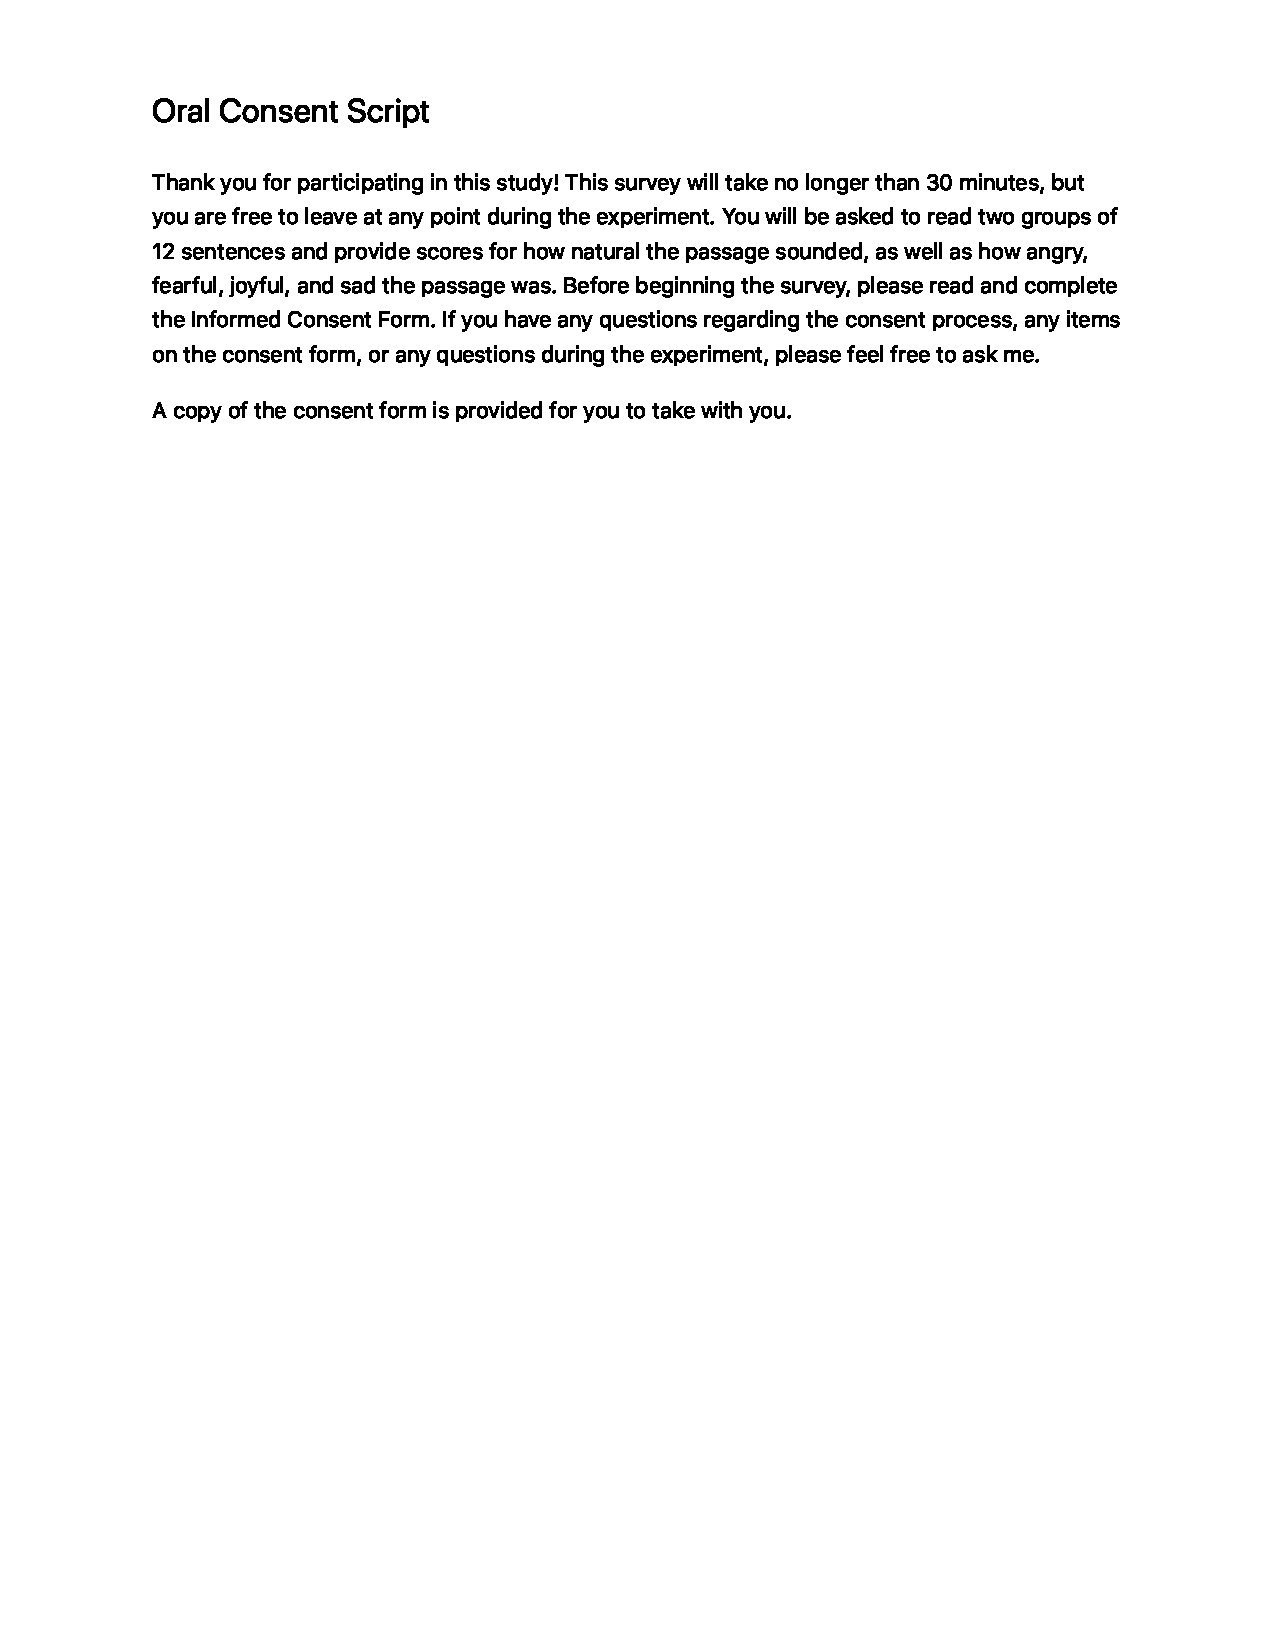
\includepdf[pages={1-},scale=0.75, pagecommand={\section{Oral Consent Script}}]{OralConsentScript.pdf}

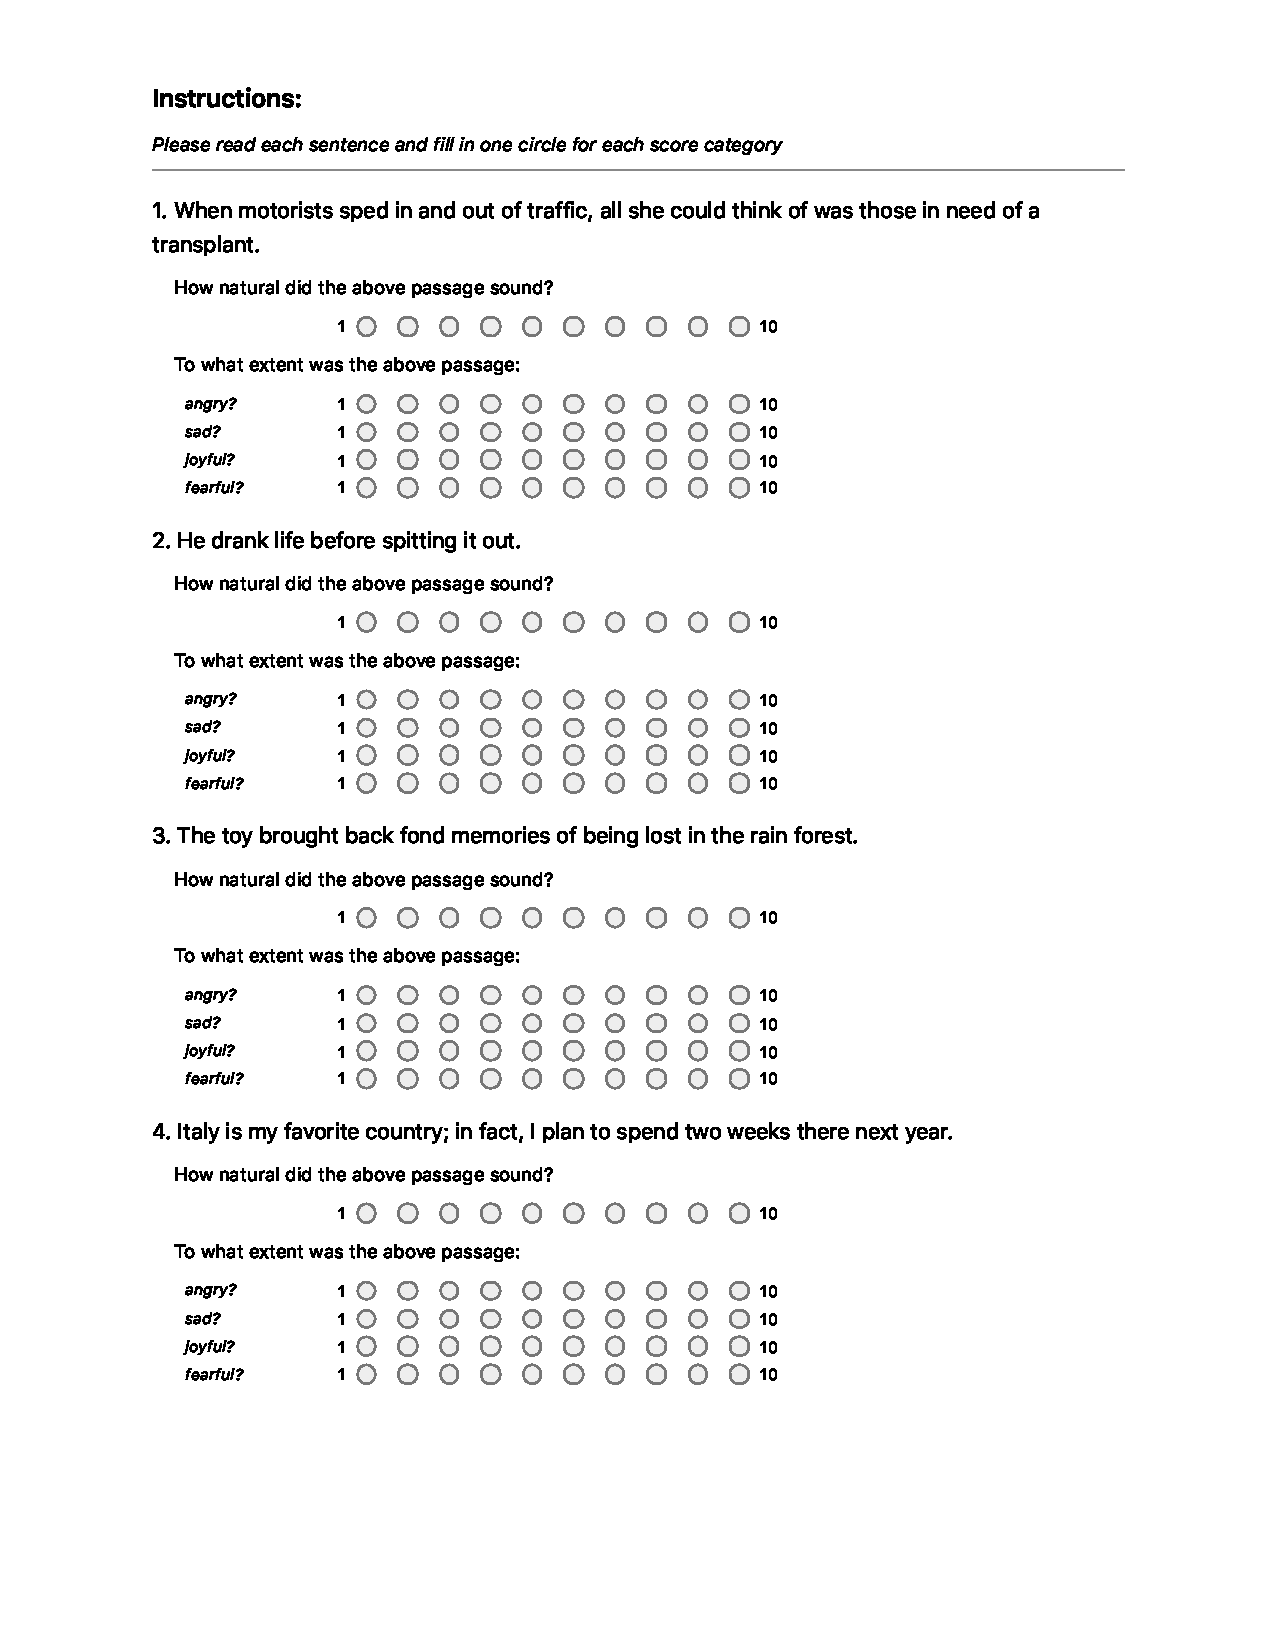
\includepdf[pages={1},scale=0.75, pagecommand={\section{Baseline Questions}}]{Baseline.pdf}
\includepdf[pages={2-},scale=0.75]{Baseline.pdf}

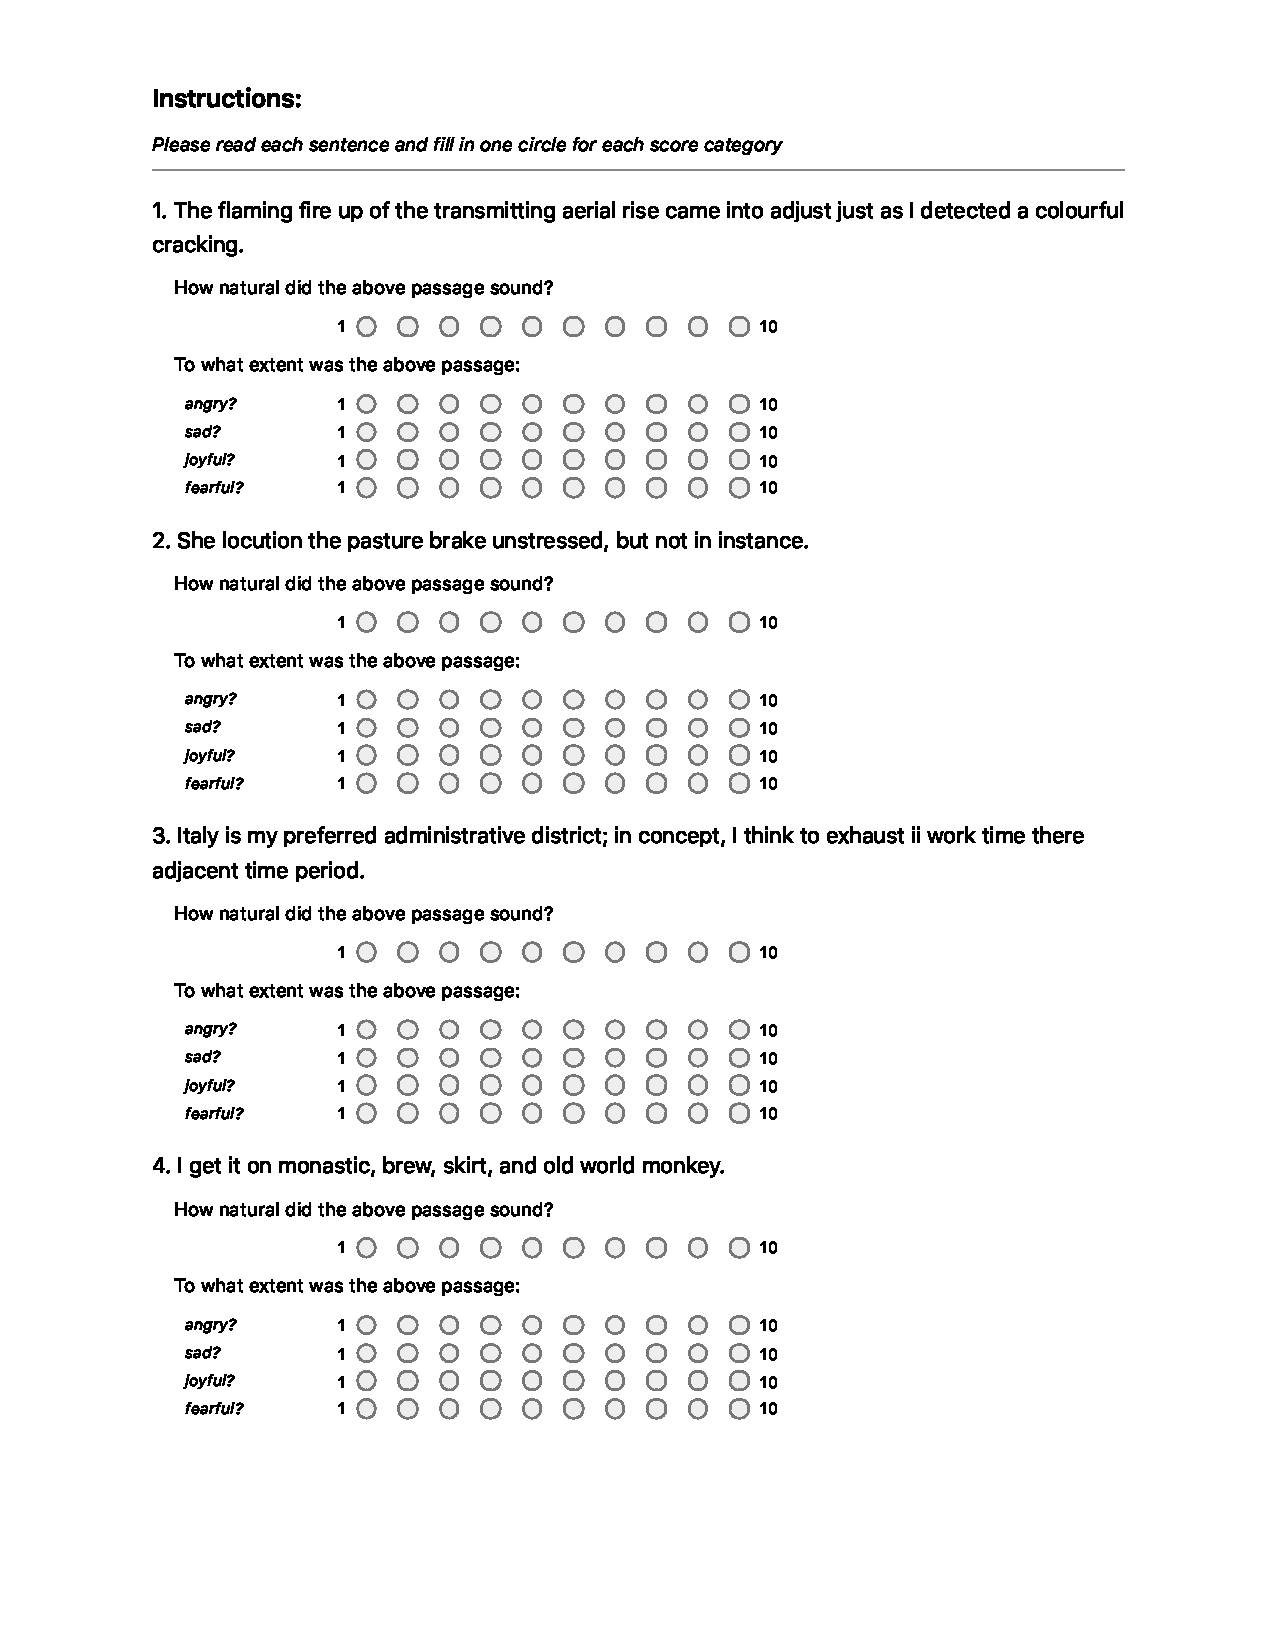
\includepdf[pages={1},scale=0.75, pagecommand={\section{Control Questions}}]{Control.pdf}
\includepdf[pages={2-},scale=0.75]{Control.pdf}

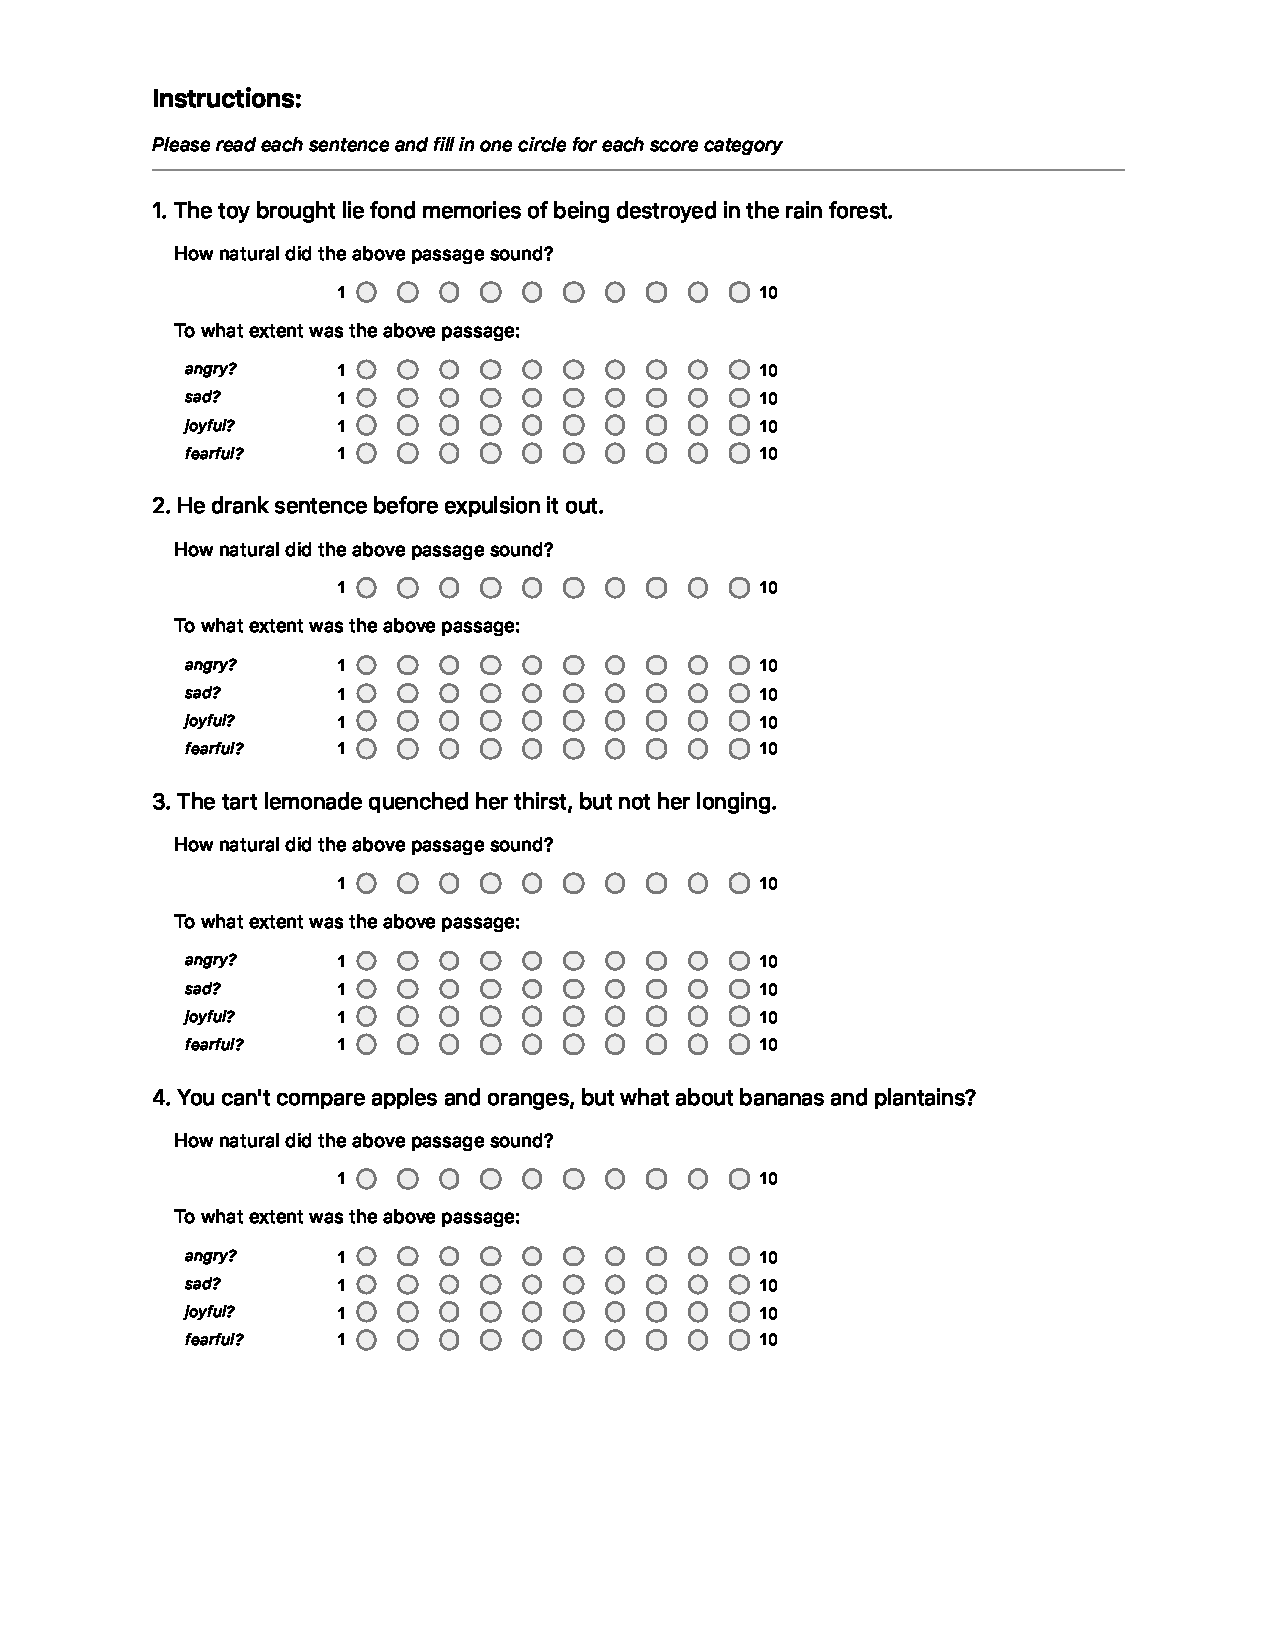
\includepdf[pages={1},scale=0.75, pagecommand={\section{Experimental Questions}}]{Experimental.pdf}
\includepdf[pages={2-},scale=0.75]{Experimental.pdf}

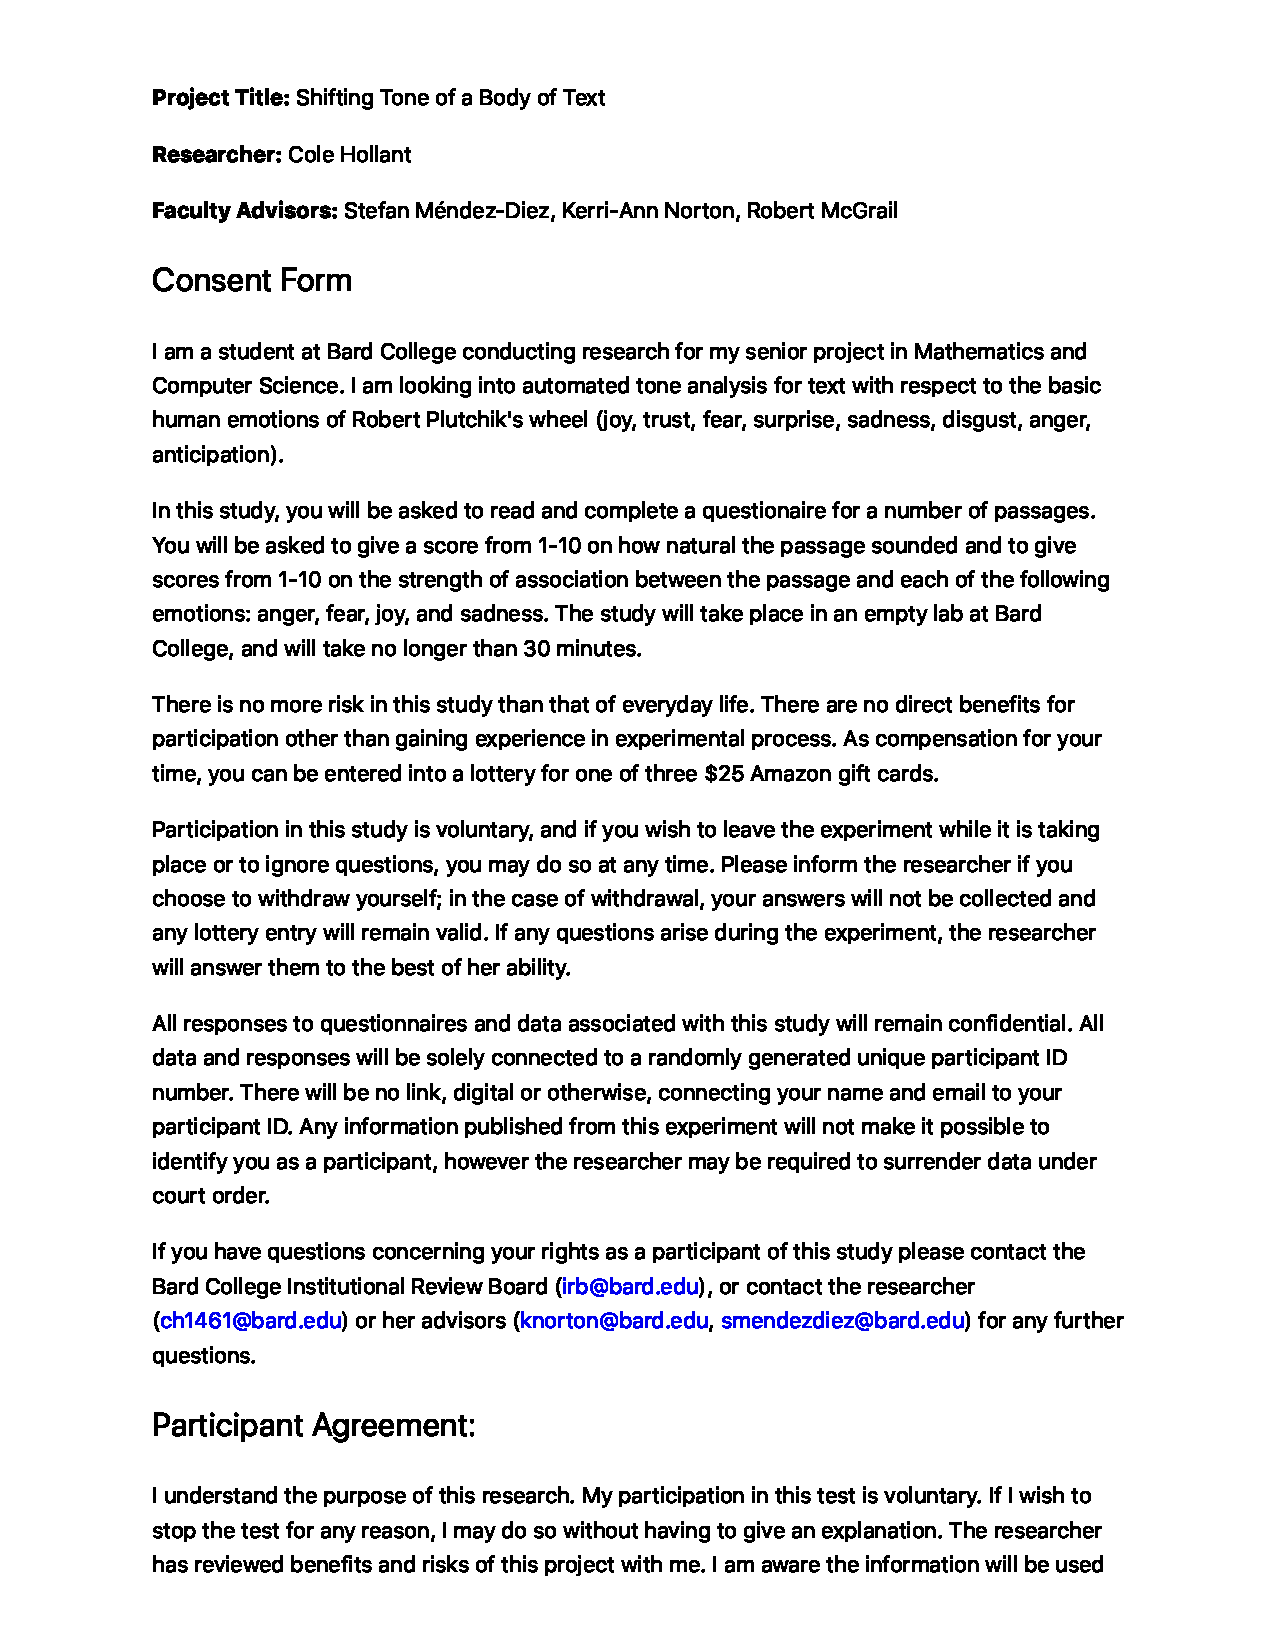
\includepdf[pages={1},scale=0.75, pagecommand={\section{Consent Form}}]{ConsentForm.pdf}
\includepdf[pages={2-},scale=0.75]{ConsentForm.pdf}

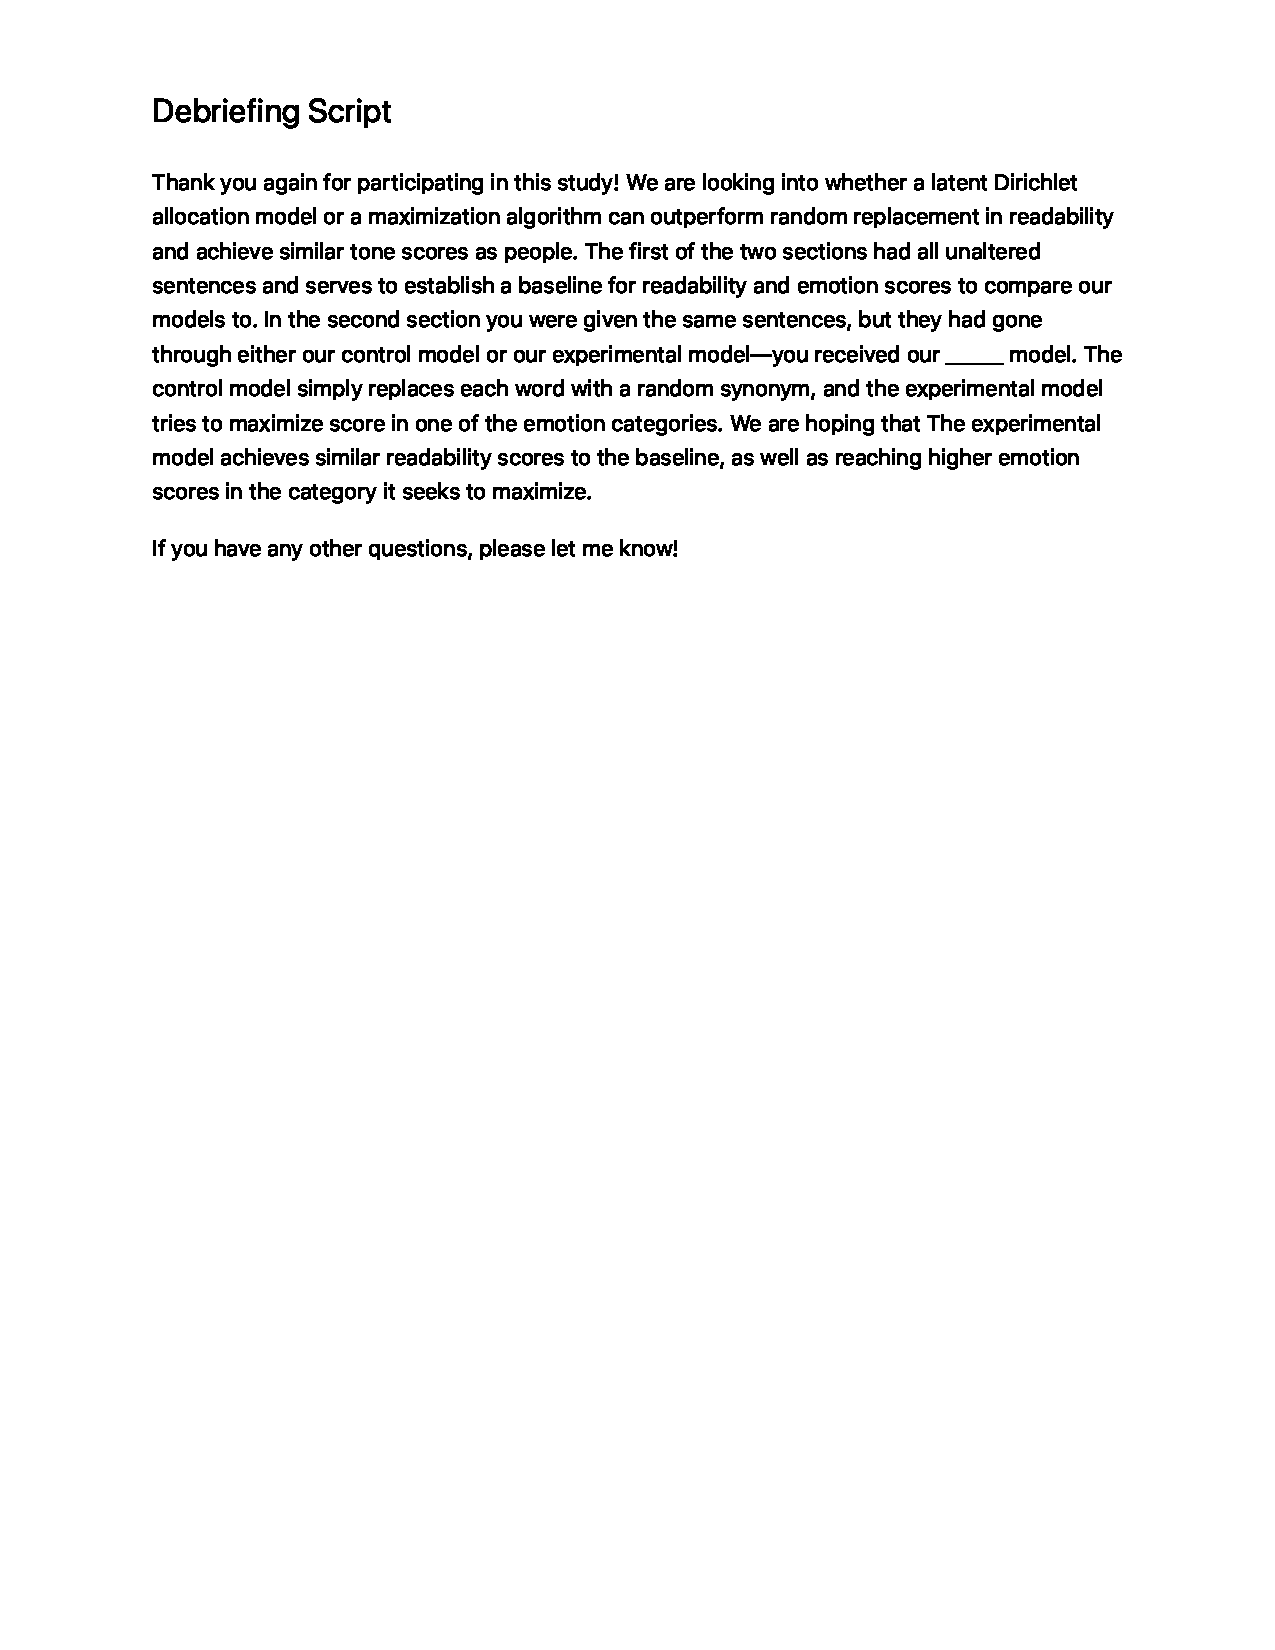
\includepdf[pages={1-},scale=0.75, pagecommand={\section{Debriefing Script}}]{DebriefingScript.pdf}

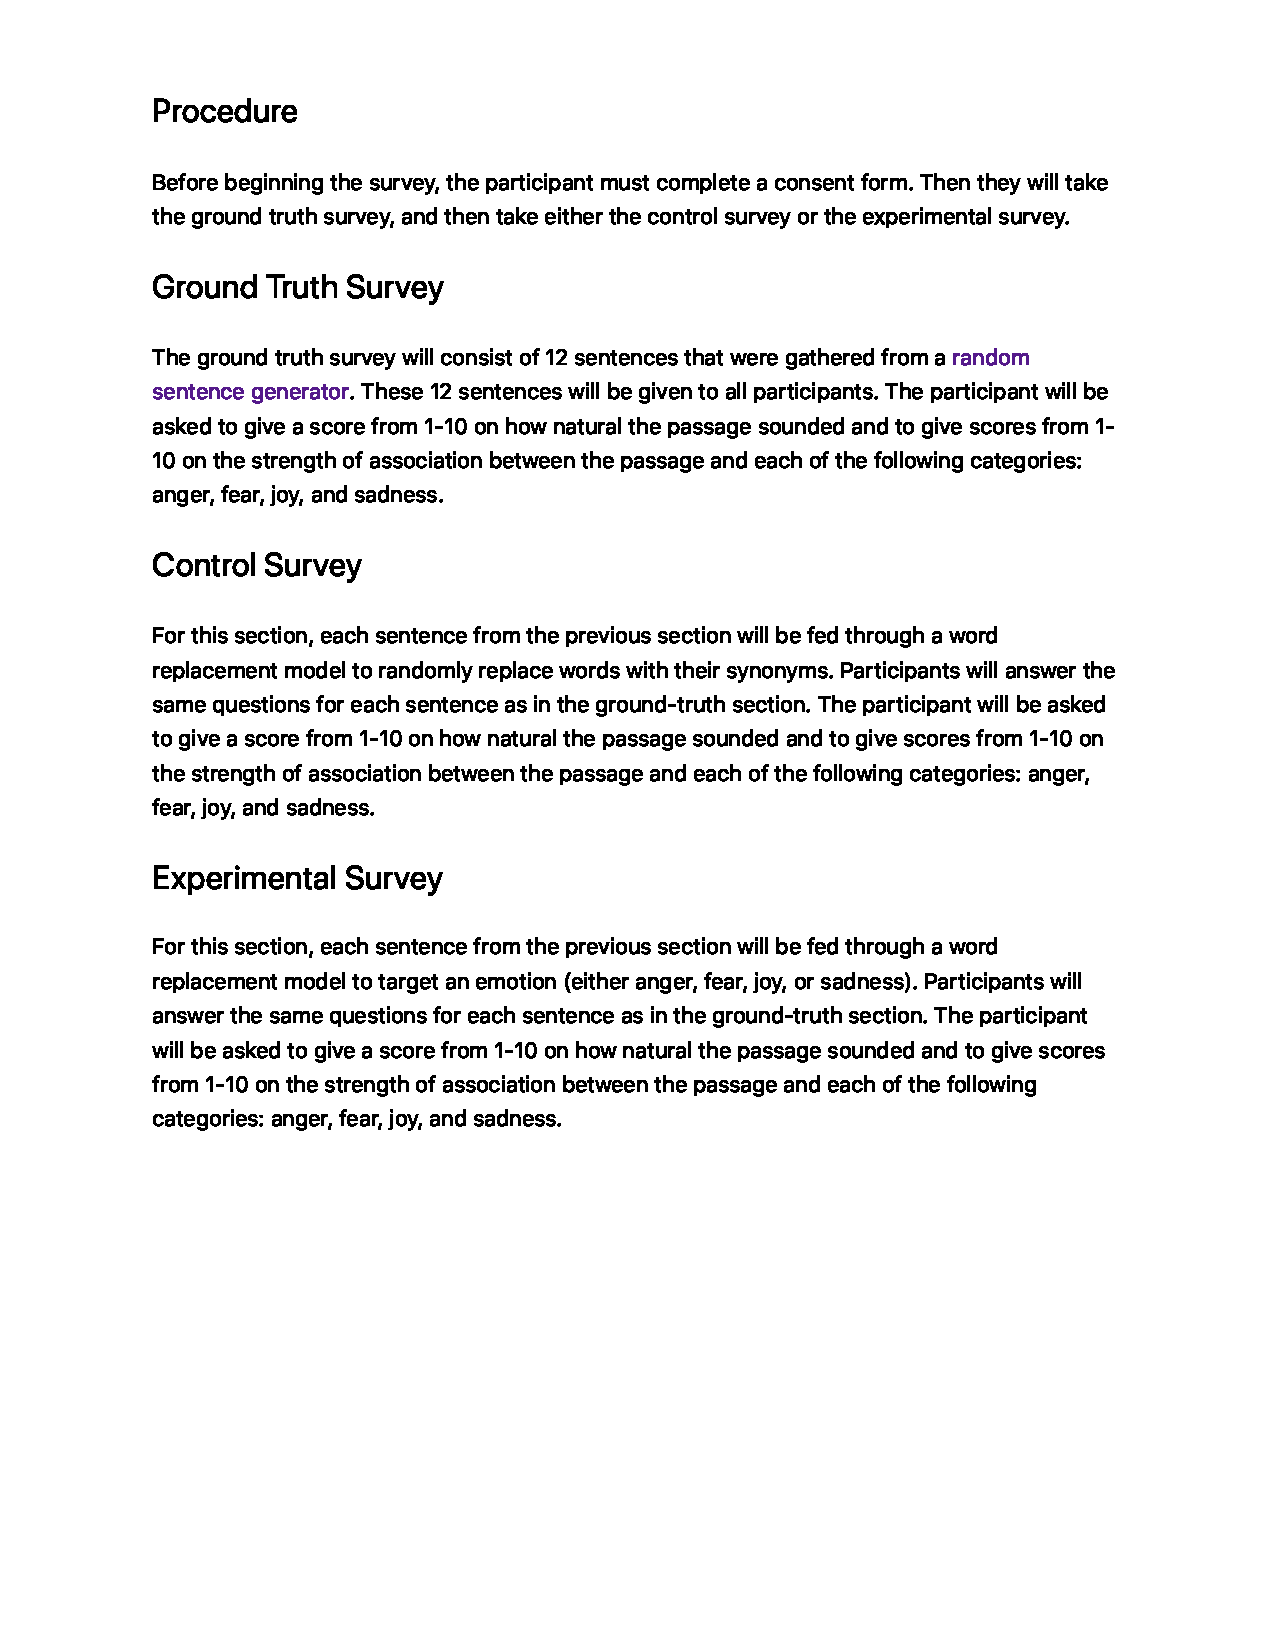
\includepdf[pages={1-},scale=0.75, pagecommand={\section{Procedure}}]{Procedure.pdf}

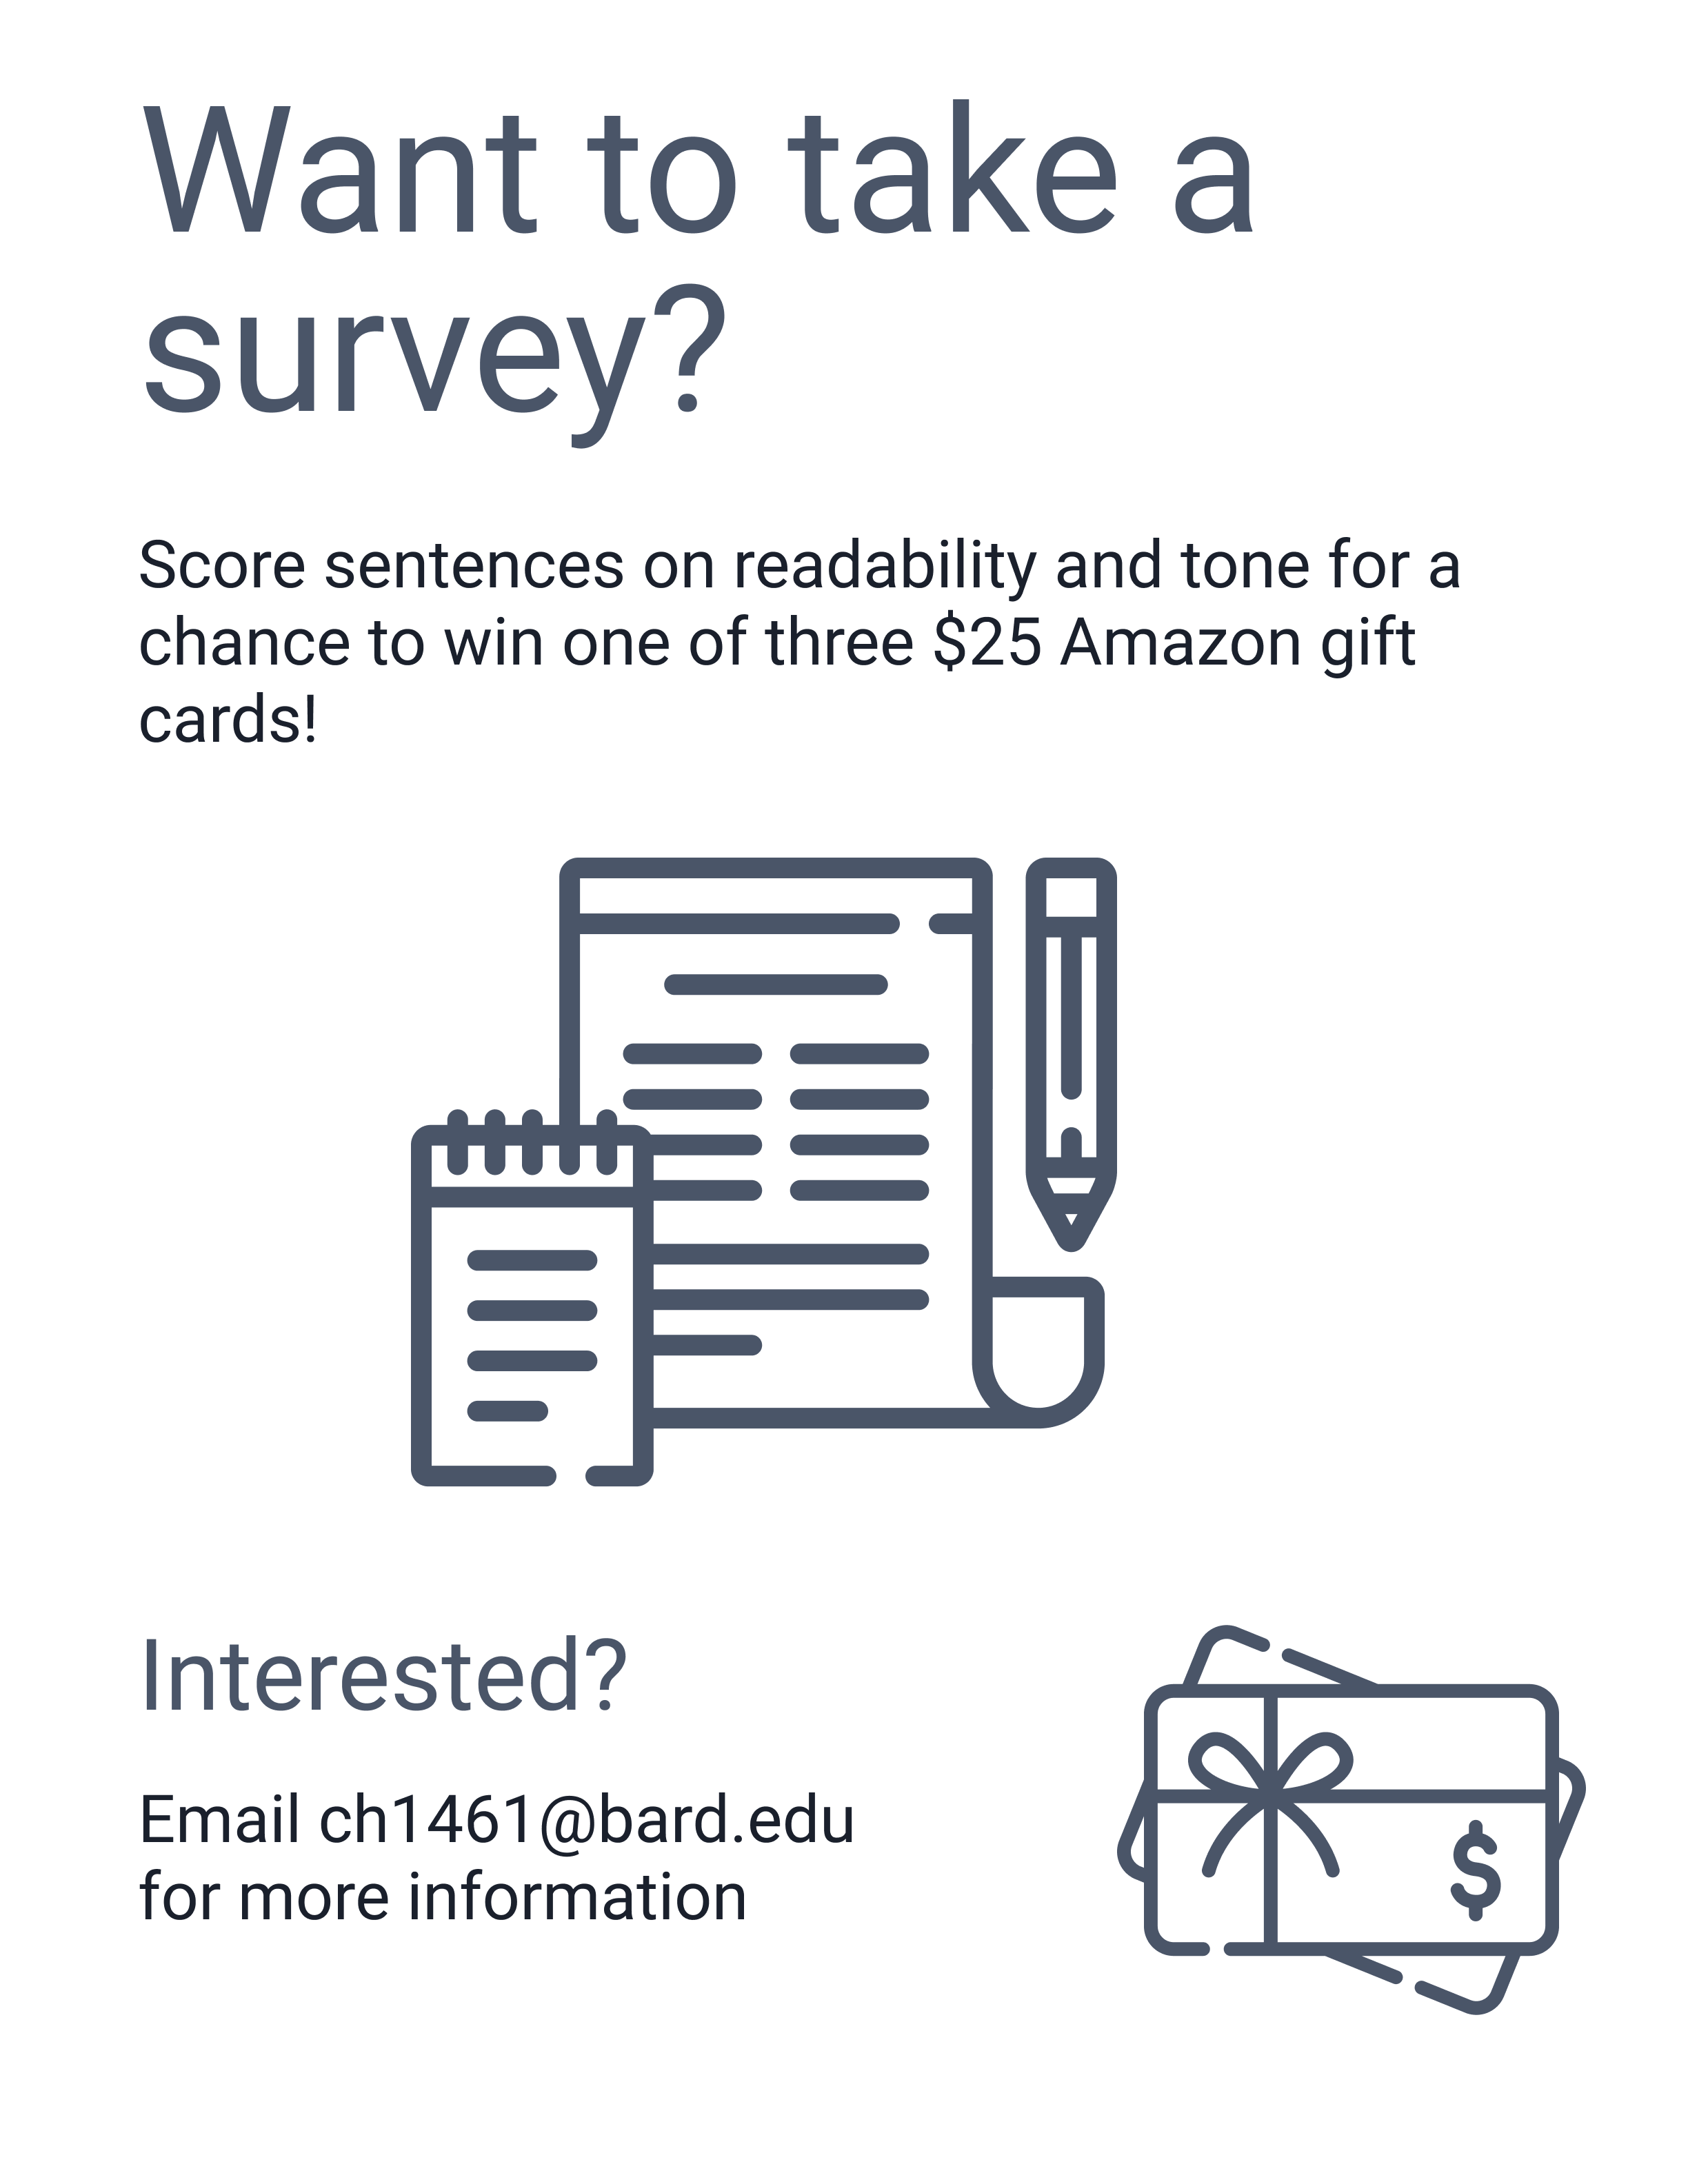
\includepdf[pages={1-},scale=0.75, pagecommand={\section{Sproj Flyer}}]{Sproj_Flyer.png}
\end{appendices}

% \nocite{*}
\bibliographystyle{plain}
\bibliography{./sproj.bib}

\end{document}

